\documentclass[output=paper]{langsci/langscibook} 
\ChapterDOI{10.5281/zenodo.1441339}
\author{Barbara Gili Fivela\affiliation{University of Salento}} 
% \chapterDOI{} %will be filled in at production
 
\abstract{The chapter aims to discuss some methods which have been adopted to perform multimodal analyses of audio-visual speech materials, focusing on linguistic distinctions conveyed by prosody. Attention is paid firstly to the production and, secondly, to the perception of speech prosody in its audio and visual dimensions. As for visual information, the paper discusses both articulatory gestures directly involved in the production of speech (e.g., lip gestures) and information that may be more traditionally considered, and referred to, as speech accompanying gestures (head movements and facial expressions). In any case, the main characteristics of the various methods are described thanks to specific examples found in the scientific literature, focusing mainly on Italian and some other Romance languages. The final goal is to highlight the advantages and disadvantages related to the specific methodological choices, clarifying the key aspects in order to make the reader able to choose among the various methods and offering the relevant references for a deeper understanding.}

 
\title{Multimodal analyses of audio-visual information: Some methods and issues in prosody research} 
\shorttitlerunninghead{Multimodal analyses of audio-visual information}
\maketitle

\begin{document} 
\label{chap:gil}\label{ch:3}
% \begin{abstract}
% \textup{Keywords: \isi{prosody} production, \isi{prosody} perception, audio-\isi{visual prosody}, bimodal, multimodal communication}
% \end{abstract}


\section{Introduction} \label{sec:gil:1}

In his 1995 work, David Crystal defines \isi{prosody} as 

\begin{quote}
a term used in SUPRASEGMENTAL PHONETICS and PHONOLOGY to refer collectively to variations in PITCH, LOUDNESS, TEMPO and RHYTHM (\citealt{Crystal1995}; capitals in the original). 
\end{quote}

The term ``\isi{prosody}'' is indeed used to refer to the modulation of the aforementioned parameters with reference to units higher than phonemes in the \isi{prosodic} hierarchy, e.g. syllables and phrases. In this respect, \isi{intonation}, stress, tone, and, for some linguists, rhythm as well, may be regarded as \isi{prosodic} features \citep{Beccaria1994}. As the above-mentioned definition highlights, \isi{prosody} is usually seen as a matter of phonetics and phonology, that is a matter of sounds, related to spoken communication. In this perspective, \isi{prosody} has often been investigated as if it was unimodal, involving sound only (to give a few examples, see the contributions related both to acoustics and perception of speech since the sixties, e.g., \citealt{Lehiste1975,Lehiste1977}). However, \isi{prosody} may be clearly expressed by means of the visual channel. In sign language; for instance, \isi{prosody} does not pertain to the sound domain as it is expressed by facial expressions, head and body movements as well as \isi{gesture duration} and tension (e.g. \citealt{Nespor1999,Wilbur2000,Sandler2005}). In similar cases, therefore, \isi{prosody} pertains to the visual rather than the audio domain.

Even though the tendency may be to treat \isi{prosody} as if it was unimodal, some investigations more easily and naturally acknowledge the multimodal character of \isi{prosody}; the fact that, in spoken communication, it usually relates to both audio and \isi{visual information}. For instance, \citet{Cave1996} recorded ten subjects while answering to yes\slash no questions and found out that a rising-falling \isi{eyebrow} movement was associated with a fundamental frequency (henceforth, F0) rise in 71\% of cases, suggesting a linguistically-driven relation between \isi{eyebrow} movement and \isi{intonation}. Other studies have shown that \isi{linguistic information} is expressed by both visual and \isi{audio information}. In fact, \isi{visual information} has been reported to be used to highlight prominent words in an utterance (\citealt{Krahmer2007,Swerts2008}) or to give positive or negative feedback \citep{Barkhuysen2005}, and  visual expressions were found to signal the end of a sentence or a speaker turn \citep{Barkhuysen2008}. Noteworthy, in various of the studies which take into account the multimodal nature of \isi{prosody}, a debated issue relates to the relevance of visual vs. \isi{audio information} in conveying \isi{prosody}. Indeed, according to some works, \isi{audio information} appears to play a crucial and major role in comparison to \isi{visual information} (e.g., \citealt{House2002,Dijkstra2006,Dohen2009,Srinivasan2003}), while in other works the relevance of audio and visual cues seems to be more balanced, and one cue appears to be somehow related to the other one (e.g. \citealt{CrespoSendra2013}) -- for details, see \sectref{sec:gil:3:1}.

In line with a traditional view of what may be of strict interest to linguistic research, investigating \isi{prosody} as if it were unimodal may be sufficient enough to shed light on the linguistic message conveyed. Indeed, felicitous communication may be just unimodal in those contexts in which either the audio or the visual signal is the only source of information (e.g., in conversations on the phone or via sign language). In general, the information in one channel is sufficient to interpret the message (e.g., it is fully included in the \isi{verbal signal} with no clear added value of multimodal analyses). Nevertheless, multimodality is often exploited and it is also very powerful in communication. Actually in some cases, both unimodal and \isi{multimodal communication} may take place simultaneously, as two different communication channels may be differently used at the same time, with a relevant impact on the message conveyed. For instance, \citet[118--119]{GiliFivela2014} discuss an example in which two local contexts\footnote{\citet{Akman.2003} propose the existence of both a global and a local context, the former corresponding to an a priori component (including, e.g., the participants’ sociolinguistic data, their respective (and mutual) knowledge\slash beliefs), the latter being constructed during the interaction and concerning linguistic (that is, knowledge of the preceding and following discourse), gestural, and action levels.} are created, with the message (and \isi{prosody} too) being conveyed in a unimodal way in one context and in a multimodal way in the other, with the result of inducing two completely different interpretations. In particular, the authors show that, in the case of a person who speaks with someone on the phone (someone who has access only to the \isi{verbal signal} in a non-face-to-face conversation) and has someone else standing in front of him\slash her (someone who has access to both audio and \isi{visual information} in a face-to-face conversation), the speaker may actually convey verbally a message to the \isi{interlocutor} on the phone while,  at the same time, denying the content of the message to the person standing in front, by means of \isi{visual information} available only to him\slash her. In a similar situation, depending on the source of information available to the \isi{interlocutor} (audio only, or audio-visual), then, the interpretation of the utterance changes as its ``truth value" is modified. In the example given by the authors, a woman is talking on the phone with an \isi{interlocutor} to whom she wants to express \isi{politeness} and a positive message, while showing to another \isi{interlocutor} standing in front of her, by means of mimicry and gestures, that the \isi{politeness} and the content of the message expressed through the phone is false. Thus, a speaker conveys two completely different meanings, being aware of the different information available in the uni- and in the \isi{multimodal communication}.\largerpage[2]

Indeed, in 

\begin{quote}
the process of understanding we do not only refer to what is said, but we also resort to a network of \isi{paralinguistic} and extralinguistic means, as those expressed by changes in \isi{prosody} (which intervenes with a crucial role […]), \isi{gesture}, gaze, smiles, laughter, and kinetic devices, such as nodding. These verbal and nonverbal means can function in an integrative or opposing way, both in assuming or negating the truth of the propositional content, and in upgrading or mitigating the related \isi{illocutionary force} (\citealt[100]{GiliFivela2014}).
\end{quote}

Therefore, the multimodality of communication (which moreover is often available even in computer mediated communication, e.g., via Skype) cannot be denied. As a matter of fact the integration of both audio and \isi{visual information} is considered here to be crucial in order to obtain a complete overview of what plays a role in both message production and interpretation. For this reason, in the following sections of this chapter the attention is focused on some methods which have been adopted in the literature on \isi{prosody} to perform multimodal investigations of speech material and are related to linguistic distinctions.\largerpage

However, before focusing on the core of the paper, several issues should be clarified. Firstly, when referring to \isi{multimodal communication}, the intent is, quite straightforwardly, to refer to the integration of verbal and visual communication, that is a communication that takes place thanks to both the \isi{verbal signal} and what we do to produce it, and the visual signal, that is what we do while producing it, which does not correspond (only) to sounds.\footnote{\label{fn:gil:2}In principle, this includes the information related to the visual context as a whole, including, but not being limited to, the speaker expressions and gestures.} In this respect, the speech sounds and their acoustic characteristics (as well as the articulatory gestures to produce them) are clearly considered as part of the verbal channel. However, articulatory gestures necessary to produce at least some sounds, that is those for which external articulators offer information (e.g. bilabials vs. non-bilabials, rounded vowels and consonants produced or affected by lip protrusion), are visible through the visual channel, although they offer information that is tightly related to the production of the \isi{verbal signal}. Finally, facial expressions, head movements and body gestures in general surely constitute a part of the visual signal that is less directly related to the mechanics of \isi{speech production} and, in a sense, for this reason represent a specific added value to \isi{multimodal communication} (adding on to the message interpretation as in the above-mentioned example). This differentiation within the \isi{visual information} available will be considered in the following sections, where, though, the attention will be restricted to gestures involving the face and head (thus not all body gestures will be considered, e.g., no hand gestures).\footnote{Given this wide view on what is relevant in the visual channel (from lip gestures needed to articulate speech to head gestures accompanying linguistic meanings), there is not one single definition of \isi{gesture} that fits the discussion. Rather, the reader is referred to the definition(s) of \isi{gesture} relevant within the various frameworks referred to in the parts of the paper.} 

Secondly, a distinction between analyses and information has to be made. Indeed, in this paper the attention is also oriented towards different types of multimodal analyses, those being the methods we use to investigate speech and \isi{prosody} (e.g., \isi{intonation}) as conveyed by more than one modality. In this respect ``multimodal'' simply indicates that more than one channel is taken into account in the analysis. However, \isi{multimodal information} (differently from analysis) corresponds to the integration of information stemming from different channels or the way the coding\slash decoding of information is affected as it happens through\slash is conveyed by different channels. Consistently, multimodal analyses and \isi{multimodal information} do not always match, as it is possible to perform, for instance, multimodal analyses of sound and speech gestures that convey either unimodal or \isi{multimodal information}. As for the former, it brings to mind investigations on \isi{prosody} and inner articulator gestures, such as that of the tongue, in which the analysis is multimodal (it relates to sound, e.g., \isi{intonation}, and \isi{visual information}, e.g., \isi{eyebrow} movements or even lip gestures), but the information offered to the \isi{interlocutor} is unimodal as conveyed\slash included in one channel only (sound); as for the latter, examples are those concerning, say, \isi{prosody} and facial expressions or \isi{prosody} and even outer articulatory gestures, in which both the analysis and the information is multimodal (it relates to both audio and \isi{visual information}).

Given these premises, in the following sections attention is concentrated on methods used for performing multimodal analyses on \isi{prosody} in speech material conveying multimodal, \isi{audio-visual information}, and in particular referring to linguistic distinctions. Methods will be described thanks to examples found in literature mainly on \ili{Italian} and some other \ili{Romance} languages. The main goal is to highlight and discuss advantages and disadvantages related to the adopted methodologies, clarifying the key aspects to allow the reader to choose from the various methods and suggesting the relevant references for their deeper understanding. The studies described also exemplify research questions which have been addressed by means of the various methods while, at the same time, offering material for discussion on advantages and disadvantages. Such discussion centers on both practical issues and on the impact of methodological choices on theoretical considerations and models that can be referred to. Attention is devoted firstly to the production of \isi{speech prosody} together with articulatory gestures, head movements and facial expressions (\sectref{sec:gil:2}) and, secondly, to the interplay of \isi{speech prosody} and visual cues in perception (\sectref{sec:gil:3}). Finally, concluding remarks complete the paper (\sectref{sec:gil:4}).


\section{Production} \label{sec:gil:2}
\subsection{Introduction} \label{sec:gil:2:1}
Multimodal analyses of \isi{speech prosody} may mainly regard the analysis of verbal speech signal including an examination of either articulatory gestures directly involved in the production of the \isi{verbal signal} or gestures which accompany the production of speech. These, while  not being directly physiologically related to the production of speech sounds, are, however, linked to the message conveyed. As for articulatory gestures directly involved in the production of the \isi{verbal signal}, think of gestures involving the lips, as external articulators, or even tongue movements (in the latter, though, gestures may be part of a multimodal analysis but are not considered as part of a message which is interpreted multimodally). Regarding gestures that accompany the production of speech, consider \isi{eyebrow} movements, as well as head position, which are not physiologically necessary for \isi{speech production}, but may be related to it and therefore may offer information to the \isi{interlocutor}. The way materials are collected and analyzed varies and depends on the type of data investigators want to focus on.\largerpage

One of the most important choices in studying \isi{multimodal communication} regards\slash relates to the way to elicit material to be investigated, exactly as it happens in unimodal investigations. In fact, the elicitation method influences the \isi{speech style} that will be focused on and, at least to a certain extent, the data that will be collected both in quantitative and qualitative terms.\footnote{To get an idea of the amount of change in \isi{prosodic} characteristics that depend on the \isi{speech style}, think, for instance, about results of comparisons of read and \isi{spontaneous speech}: the latter shows more syllables produced per second and, on average, a wider F0 range \citep{Blaauw1995} as well as a high number of rising boundaries (\citealt{Ayers1994,Blaauw1995}).} In investigating linguistic \isi{prosody} in \isi{speech production} within a multimodal perspective, the choice often regards very controlled speech styles, obtained by eliciting isolated sentences or sentences in context (e.g., short dialogues inducing the intended \isi{pragmatic interpretation} on the target utterance\slash word), including target words or pseudowords. In fact, methods to elicit more spontaneous-like speech styles are not significantly considered in the literature on multimodal analyses of \isi{multimodal communication}, even though the scientific community has been quite recently taking them into account at least for investigating unimodal communication (e.g.,  recordings of \isi{semi-spontaneous speech}, such as Map Task (\citealt{Brown1983,Anderson1991}), spot-the-difference dialogues (\citealt{Savy2009,Pean.1993}) or even possibly more \isi{spontaneous speech}, such as that obtained by means of the Discourse Completion Task (\citealt{BlumKulka1989}, \citeauthor{Vanrell.2018}, this volume) or dialogues (e.g., \citealt{Geng2013}). 

In any case, the choice of \isi{speech style} is heavily influenced by the type of data to be collected, as  will be discussed in the following section with particular reference to tracking and imaging data.


 
\subsection{Methods for data collection and analysis: some examples} \label{sec:gil:2:2}


In works which adopt a multimodal perspective, data collection usually involves the recording of verbal signals simultaneously with tracking or imaging data. 

Tracking data are those collected by recording the position in time of specific markers. They are usually collected by means of either optotracking systems, exploiting cameras that record the infrared 3D signal reflected by markers glued on the speaker face (e.g., \is{eyebrow}eyebrows, lips), or systems recording the position in time of electrodes that are placed within an appropriate electromagnetic field. In the latter, recording takes place by means of systems such as magnetometers or electromagnetic articulographs that work thanks to electrodes that may be glued both on the speaker’s face and in the speaker’s mouth (e.g., \is{eyebrow}eyebrows, lips, tongue). Independently of the system adopted, the procedure consists of gluing markers\slash electrodes on the articulators to track, using three stable positions (usually behind the ears and either on the nose or, if possible, on the upper incisors) for head position normalization. In all cases, the corpus recorded is usually highly controlled, the number of repetitions recorded for each item and speaker is quite high (e.g., 7 to 10), while the number of subjects is limited (it was even one in earlier studies, but is increasing and now may reach even 10, at least in the case quite recent recording systems are adopted). Various research questions on \isi{prosody} have been answered by collecting such kind of data. 

For instance, \citet{Avesani2007,Avesani2009} investigate the accent-induced articulatory strengthening, focusing on the kinematics of lip movements in the production of syllables which are variably prominent, being unstressed, stressed and nuclearly accented. They collect articulatory data by means of ELITE, an automatic optotracking movement analyzer, which allows 3D kinematic data acquisition and synchronous recording of the acoustic signal. Markers considered for the analysis are those glued on the lower and upper lip, and on both the tip of the nose and the earlobes for head position normalization. Eight repetitions are recorded of nonce-words (CVCV(C)CV, where C = [b, m]; V=[a, i]) produced by two female speakers (of two varieties of \ili{Italian}). The target words are inserted in \isi{declarative} sentences in short dialogues to elicit the intended interpretation, so that the \isi{penultimate syllable} of the nonce-words can be unstressed, stressed or nuclearly accented in a contrastively focused constituent.\pagebreak

\begin{figure}[b]
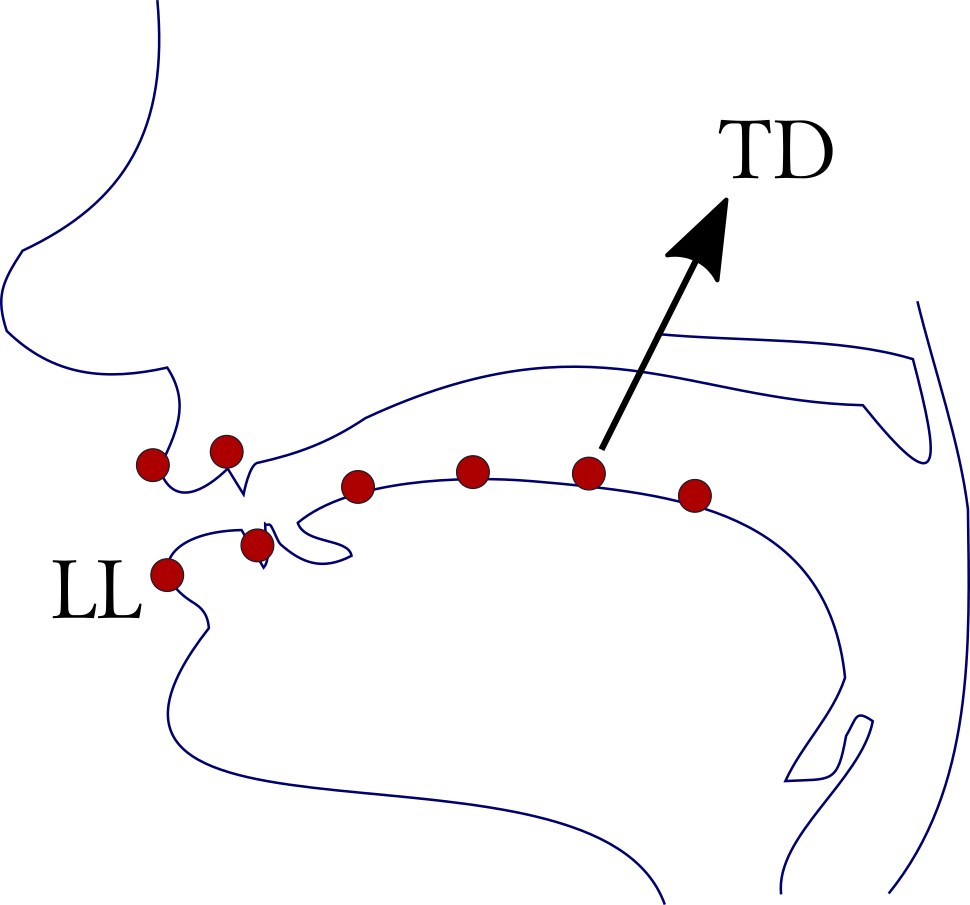
\includegraphics[width=0.5\textwidth]{figures/GIL-img1.png}
\caption{Sensors glued on the articulators; LL and TD stand for Lower Lip and Tongue Dorsum, respectively.}
\label{fig:gil:1} 
\end{figure}
 
 
To make a slightly different example that relates to \isi{intonation}, in \citet{Stella2014} articulatory differences in the alignment of the L+H* \isi{pitch accent} with the lip gestures are investigated, focusing on the \isi{syllable} [ma] in three different languages, that is \ili{Italian}, \ili{Spanish} and \ili{Catalan}. In such languages, in fact, the L+H* \isi{pitch accent} conveys different pragmatic functions, as it expresses a narrow-\is{focus!contrastive}contrastive focus in the latter two languages while it is non-focal in the former; the goal is then to check if there are differences in the phasing of the acoustic rise (L+H*, produced by a rising laryngeal \isi{gesture}) with the lip gestures to produce [ma]. In this work, an AG500 \isi{articulograph} is used to track speech gestures (simultaneously with the acoustic signal registration), by gluing 4 sensors on the tongue, 2 on upper and lower lips (see \figref{fig:gil:1}), 2 on upper and lower incisors and 2 behind the ears, for head movement normalization. The authors record 8 speakers in total, and ask them to produce 10 repetitions of a corpus composed by pseudowords such as [mi.ˈma.mi] and [mi.ˈma.mi.ma]. Target words are inserted in dialogues consisting of two question-answer exchanges, built in such a way that the answers including \isi{declarative} sentences with non-focal or \is{focus!contrastive}contrastive correction focus in a \isi{prenuclear position}. 



Under imaging data, a set of quite different techniques may be included, ranging from the video recording of speakers (e.g., her\slash his head, half of her\slash his body; \citealt{Ekman1978}) to the collection of, say, tongue imaging data during \isi{speech production} (by means of ultrasound systems; \citealt{Stone2005}). Of course, investigating what happens inside the mouth, as already mentioned, may be more useful for a multimodal analysis of \isi{speech production} rather than for an analysis of \isi{multimodal information} in speech communication and, therefore, will not be further discussed in this paper. However, when considering the collection of speech data together with the video of, say, the speaker’s head, the method for data collection is quite straightforward and consists of recording audio and video simultaneously, obtaining time aligned audio and video materials. Digital cameras are used for audio-video recordings, with the highest frame rate per second possible. In the case of these methods too, various research questions may be addressed. 
 

For instance, \citet{CrespoSendra2013} collect audio-video material in order to investigate (also perceptually) the interaction between \isi{intonation} and facial gestures in the expression of  information-seeking and incredulity yes\slash no questions in \ili{Catalan} and Dutch. They perform audio-video recordings of 5 subjects for each language thanks to a digital camera that records (25 frames per second) the upper body and face of subjects. Participants are asked to read (for ten times) “in an expressive fashion” the target sentences inserted in dialogues inducing the two intended interpretations of yes\slash no questions.

To offer another example, \citet{GiliFivela2015informazionimultimodali} also exploits the use of a digital camera to acquire both audio and video signals (the upper body and face – see \figref{fig:gil:2}) while 5 subjects read aloud, for at least five times, short discourses aimed to simulate a {Discourse Completion Task} (\citealt{BlumKulka1989}, \citeauthor{Vanrell.2018}, this volume).\footnote{The simulation consisted in having the subjects memorize the target sentence that was proposed within various  contexts used to induce the different interpretations. This procedure was needed to create a communication context that was as natural as possible, though the sentence structure and composition could not be left to the speaker’s choice. Such high control on the productions was necessary as, at a later stage of investigation, various combinations of audio and video signals had to be matched  (see below).} In this work, facial expressions and head movements are investigated across sentence modalities, considering statements, wh-questions and exclamations with the aim to check if \isi{visual information} could be more important for the message interpretation when it represented non-neutral, thus marked, information (e.g., in wh-questions conveying surprise or in exclamations vs. neutral statements).

  

\begin{figure}
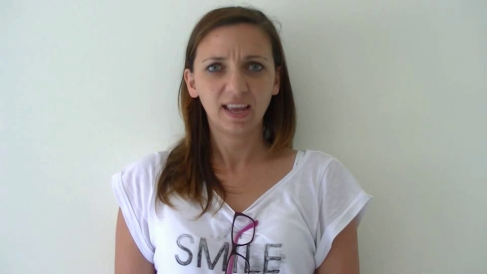
\includegraphics[height=.3\textheight]{figures/GIL-img2.png}

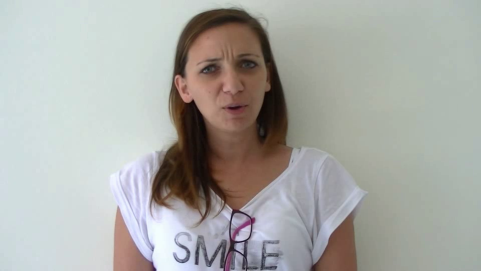
\includegraphics[height=.3\textheight]{figures/GIL-img3.png}

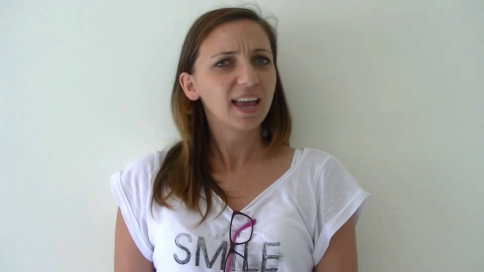
\includegraphics[height=.3\textheight]{figures/GIL-img4.png}
\caption{Examples of snapshots taken from the recording of a surprised wh-question (from the corpus used in \citealt{GiliFivela2015informazionimultimodali}); changes in visual information is clearly detectable.}
\label{fig:gil:2}
\end{figure} 

Let’s now turn to discussing methods adopted for analysis. Data analysis, as expected, changes depending on data collection, though, when the goal is to perform multimodal analysis of \isi{multimodal information} related to \isi{prosody}, the analysis usually concerns both the verbal and the visual modalities. 

Methods used for analysing speech sounds are assessed, due to the long tradition of studies focused on both qualitative and quantitative aspects. In fact, since the 60s, \isi{speech prosody} has been studied by performing acoustic measurements of various parameters, such as duration, F0, intensity. However, especially when \isi{linguistic information} is at issue, the analysis usually involves qualitative evaluations too, that stem from examination aiming to highlight the existence of linguistic categories out of the variation of \isi{phonetic} parameters. In the case of \isi{prosody}, and particularly in the case of \isi{intonation}, this is true, for instance, for all the works whose goal is the identification of phonological categories within the Autosegmental-Metrical theory (\citealt{Pierrehumbert1980,Ladd.1996,Beckman1997}). Methods adopted for these purposes are not particularly new to the field of \ili{Romance} linguistics or even general linguistics and therefore will not be discussed in detail here. 

As for \isi{visual information} in the production of clearly \isi{linguistic information} (e.g., \isi{prosodic} focus, \isi{sentence modality}) the situation is more heterogeneous. On the one hand, a relatively long tradition of studies has systematically investigated \isi{speech production} and the synchronization of acoustic signal and articulatory movements\slash gestures. These works have focused on speech articulatory gestures as a whole, rather than on \isi{visual information}, and were inspired for instance by Browman and Goldstein’s proposal within the task dynamics (\citealt{Browman1984,Browman1985}; for \isi{prosody}, e.g. \citealt{Edwards1991,Beckman1992} and following works on jaw movements related to \isi{prosodic} structure \citealt{Byrd1998,Byrd2003}; see also \citealt{GiliFivela2008book} and \citealt{Avesani2007}, as mentioned above; for \isi{intonation}, \citealt{DImperio.2007,PrietoETAL2007,Muecke2009}). Though the focus of such works is not on \isi{visual information}, \isi{lip movement} is quite often focused on, which may also be seen as a relevant part of \isi{visual information} related to speech and \isi{speech prosody}. The analysis usually regards the vertical or the horizontal movement of markers\slash electrodes whose position was previously recorded. In some cases, analyses relate to the position of specific electrodes (e.g. the one glued on the lower lip), while in other cases it may already be related to derived measures (e.g., a track corresponding to the lip aperture signal — i.e. to the distance between the positions recorded for the two lips — is directly taken into account). In any case, relevant landmarks are identified in the labelling phase (e.g., onset and offset of gestures on the position track, at the zero-crossings in the corresponding velocity signals; the velocity peak of gestures on the velocity track) and measures are taken of their temporal (ms) and spatial (mm) characteristics. These measures allow then to calculate other, derived, measures, such as \isi{gesture duration} and displacement or \isi{gesture} stiffness (as the ratio between \isi{peak velocity} and displacement). Statistical analysis is then performed on these measures and usually also related to more traditional acoustic measures performed on the very same recordings (as audio was simultaneously recorded).

The usual method adopted in similar investigations may be exemplified by taking into account one of the foundational works concerning \isi{prosody}. \citet{Byrd1998} analyze kinematic data by three subjects to check, among other things,

\begin{quote}
whether multiple levels of \isi{prosodic} boundaries can be distinguished in the spatio-temporal patterning of articulation (\citealt{Byrd1998}: 173).
\end{quote}

They basically look at the articulatory correlates of final lengthening, a phenomenon which had already been found acoustically by the end of \isi{prosodic} constituents (\citealt{Oller1973,Wightman1992}). In order to achieve their goal, the authors record a CV sequence within which five different \isi{prosodic} boundaries were realized. By means of a magnetometer system (EMMA, by \citealt{Perkell1992}), the authors record the horizontal and vertical position of two electrodes glued on the upper lip and the lower lip, and, after the recordings, calculate the Lip Aperture signal as corresponding to the Euclidean distance between the two lips. By means of a software dedicated to signal processing (HADES, \citealt{Rubin1995}) they automatically mark (at the zero-crossings in the corresponding velocity signals) the onset\slash offset of the lip closing\slash opening movement for each of the consonants in the target sequence. On the basis of the movement onset, peak, offset, and movement \isi{peak velocity} the authors calculate a number of dependent variables, such as the duration of the \isi{pre-boundary opening} and \isi{post-boundary closing} movement and of the transboundary interval (that is, the duration of \isi{pre-boundary opening} and \isi{post-boundary closing}; \citealt{Byrd1998}: 179). Articulatory data, together with data concerning the acoustic characteristics of the sequences under investigation allow the authors to show, for instance, that three levels of \isi{prosodic} boundaries may be statistically distinguished by the temporal and spatial characteristics of lip gestures which are adjacent to the boundaries (e.g., by the lengthening of the \isi{pre-boundary opening} movements and mainly by the lengthening of \isi{post-boundary closing} movements). 

Along similar lines, though the kinematic data were acquired by means of an optotrack system, \citet{Avesani2007,Avesani2009} analyze data on accent-induced articulatory strengthening, as already mentioned. They label and measure acoustic data by means of \isi{Praat} (\citealt{Boersma.praat}) while articulatory data are analyzed by means of \textit{Interface} \citep{Tisato2005}. To offer more details on the analysis phase, it is worth to recall that, firstly, the authors check each utterance for the realization of pitch accents on the target syllables; secondly, they center their attention on the lip aperture and take spatial (mm) and temporal (ms) measures of the onset, the target and the \isi{peak velocity} of both the opening and the closing gestures. They then calculate various dependent measures, such as \isi{gesture duration}, its displacement, \isi{peak velocity}, time-to-\isi{peak velocity} (which is the duration of the acceleration phase) and \isi{gesture} stiffness (as the ratio between \isi{peak velocity} and displacement). By statistically analyzing acoustic and articulatory data the authors show, among other things, that in the production of one speaker:

\begin{quote}
compared to stressed, unstressed syllables show shorter acoustic and articulatory duration, smaller displacement, equal \isi{peak velocity}, shorter TTP and higher stiffness for both opening and closing gestures (\citealt[983]{Avesani2007}).
\end{quote}

The authors observe that, for the same speaker, a dynamic mechanism of linear rescaling seems to take place when accented syllables rather than stressed syllables were taken into account. However, for the other speaker different dynamics seem to characterize gestures when considering different levels of \isi{prominence}, that is linear rescaling does not seem to necessarily take place.

Other studies adopt very similar methods to investigate \isi{intonation}, and in particular the intergestural coordination between laryngeal and supralaryngeal gestures. In fact, tonal alignment may be investigated as a matter of coordination between gestures to produce F0 modulation and gestures to produce segments, syllables or other units, that is as a coupling of tonal and oral gestures (\citealt{DImperio2002,Ladd2008,PrietoTorreira2007}). For instance, the investigation on \ili{Italian}, \ili{Catalan} and \ili{Spanish} by \citet{Stella2014} mentioned above may help in exemplifying the methods exploited in the analysis. To perform their analysis the authors label tonal targets and segmental boundaries by means of a \isi{Praat} script and label the articulatory data by means of a MatLab graphical user interface-based software for multimodal articulatory data inspection and analysis, MAYDAY \citep{Sigona2015}. The \isi{Praat} TextGrids, containing segmental and tonal labels, are imported in MAYDAY, where the articulatory data are then semi-automatically labelled, marking the onset, offset and \isi{peak velocity} of each opening and closing \isi{gesture} realized to produce the CV target sequence in the target words. Latencies between tonal targets and articulatory landmarks are then computed by means of a MatLab script. The method described so far may be considered to be quite traditional (apart from the choice in the software and scripts to label and measure the articulatory data, which pretty much varies depending on the laboratory and research group). What is worth mentioning as for the methodological choices is that, rather than just analyzing measures by means of statistics to identify significant differences, in this work a MatLab script is also implemented and used to obtain graphical plots of the alignment patterns in order to visually inspect the timing relations between tonal and oral gestures. The graphical plot of the alignment patterns is based on the mean temporal values for the 10 repetitions analyzed for each item (that is for each speaker, each \isi{syllable} and word stress type). As shown in \figref{fig:gil:3}, the alignment plot is formed by 4 tiers (Segments, Tones, Lower Lip and Tongue Dorsum), showing the temporal values of articulatory, segmental and tonal landmarks normalized at the onset of the target word. Visual inspection of the alignment patterns and two-way ANOVA allow the authors to highlight the quite stable alignment of tonal targets with articulatory landmarks. 

To conclude, methods used in the analysis of the interplay between gestures for producing speech and acoustic features of speech are quite well known, \linebreak though there are not many works adopting such methods to deal with \isi{prosody} in \ili{Romance} languages. 


\begin{figure}
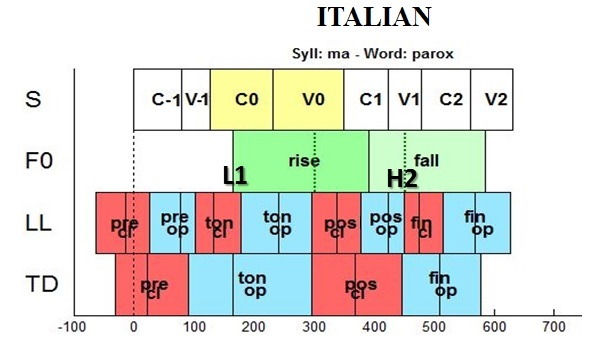
\includegraphics[width=\textwidth]{figures/GIL-img5.jpg}
\caption{Patterns of alignment of L+H* productions in Italian (see also \citealt{Stella2014}); the 4 tiers in the alignment plot (from top to bottom, Segments, Tonal events, Lower Lip and Tongue Dorsum) show the temporal values of articulatory, segmental and tonal landmarks normalized at the onset of the target word.}
\label{fig:gil:3}
\end{figure}\pagebreak

On the other hand, interest in the production of \isi{visual information} which is not directly related to the articulation of speech units (that is, it is not physiologically related to the production of speech sounds, but rather to the message conveyed) is even more rare in investigations related to the linguistic message. In fact, methods for investigating \isi{visual information} in communication are assessed, but intensive studies on the role of such information in the coding and decoding of linguistic \isi{prosody} and message have definitely not been a top priority (see \sectref{sec:gil:1}).

In the early 80s a system to code facial expressions and head movements was proposed by Ekman (\citealt{Ekman1978,Ekman2002}) and it is still used nowadays. The system is called the \textit{Facial Action Coding System} (FACS) and it identifies \textit{Action Units} (AUs), corresponding to the activation of one or more muscles producing a change in the facial appearance. AUs are identified by numbers (letters+numbers in some cases) and names (e.g., AU 4 – \textit{Brow Lowerer}): the former are basically arbitrary and their association to names helps in learning the coding system, even though the actual coding by experienced coders refer to numbers rather than names. The coding is basically performed by observing movements of the skin, specific parts of the face (to start with the coder’s own face in the learning phase) and the head. Indeed, these movements allow to identify the appropriate AU that took place and to code it appropriately together with a score of its intensity. Indeed,  AUs and their combinations can be described also in terms of intensity levels (from A, that is “trace”, to E, that corresponds to “maximum”). For instance, the images reported in \figref{fig:gil:4}, starting from top to bottom may be labelled as AU4 \textit{Brow Lowerer}, AU4+7 \textit{Brow Lowerer} + \textit{Lid Tightener} and AU2 - \textit{Outer Brow Raiser}; their intensity level may be labelled as \textit{C- Marked or Pronounced}.

 

\begin{figure}
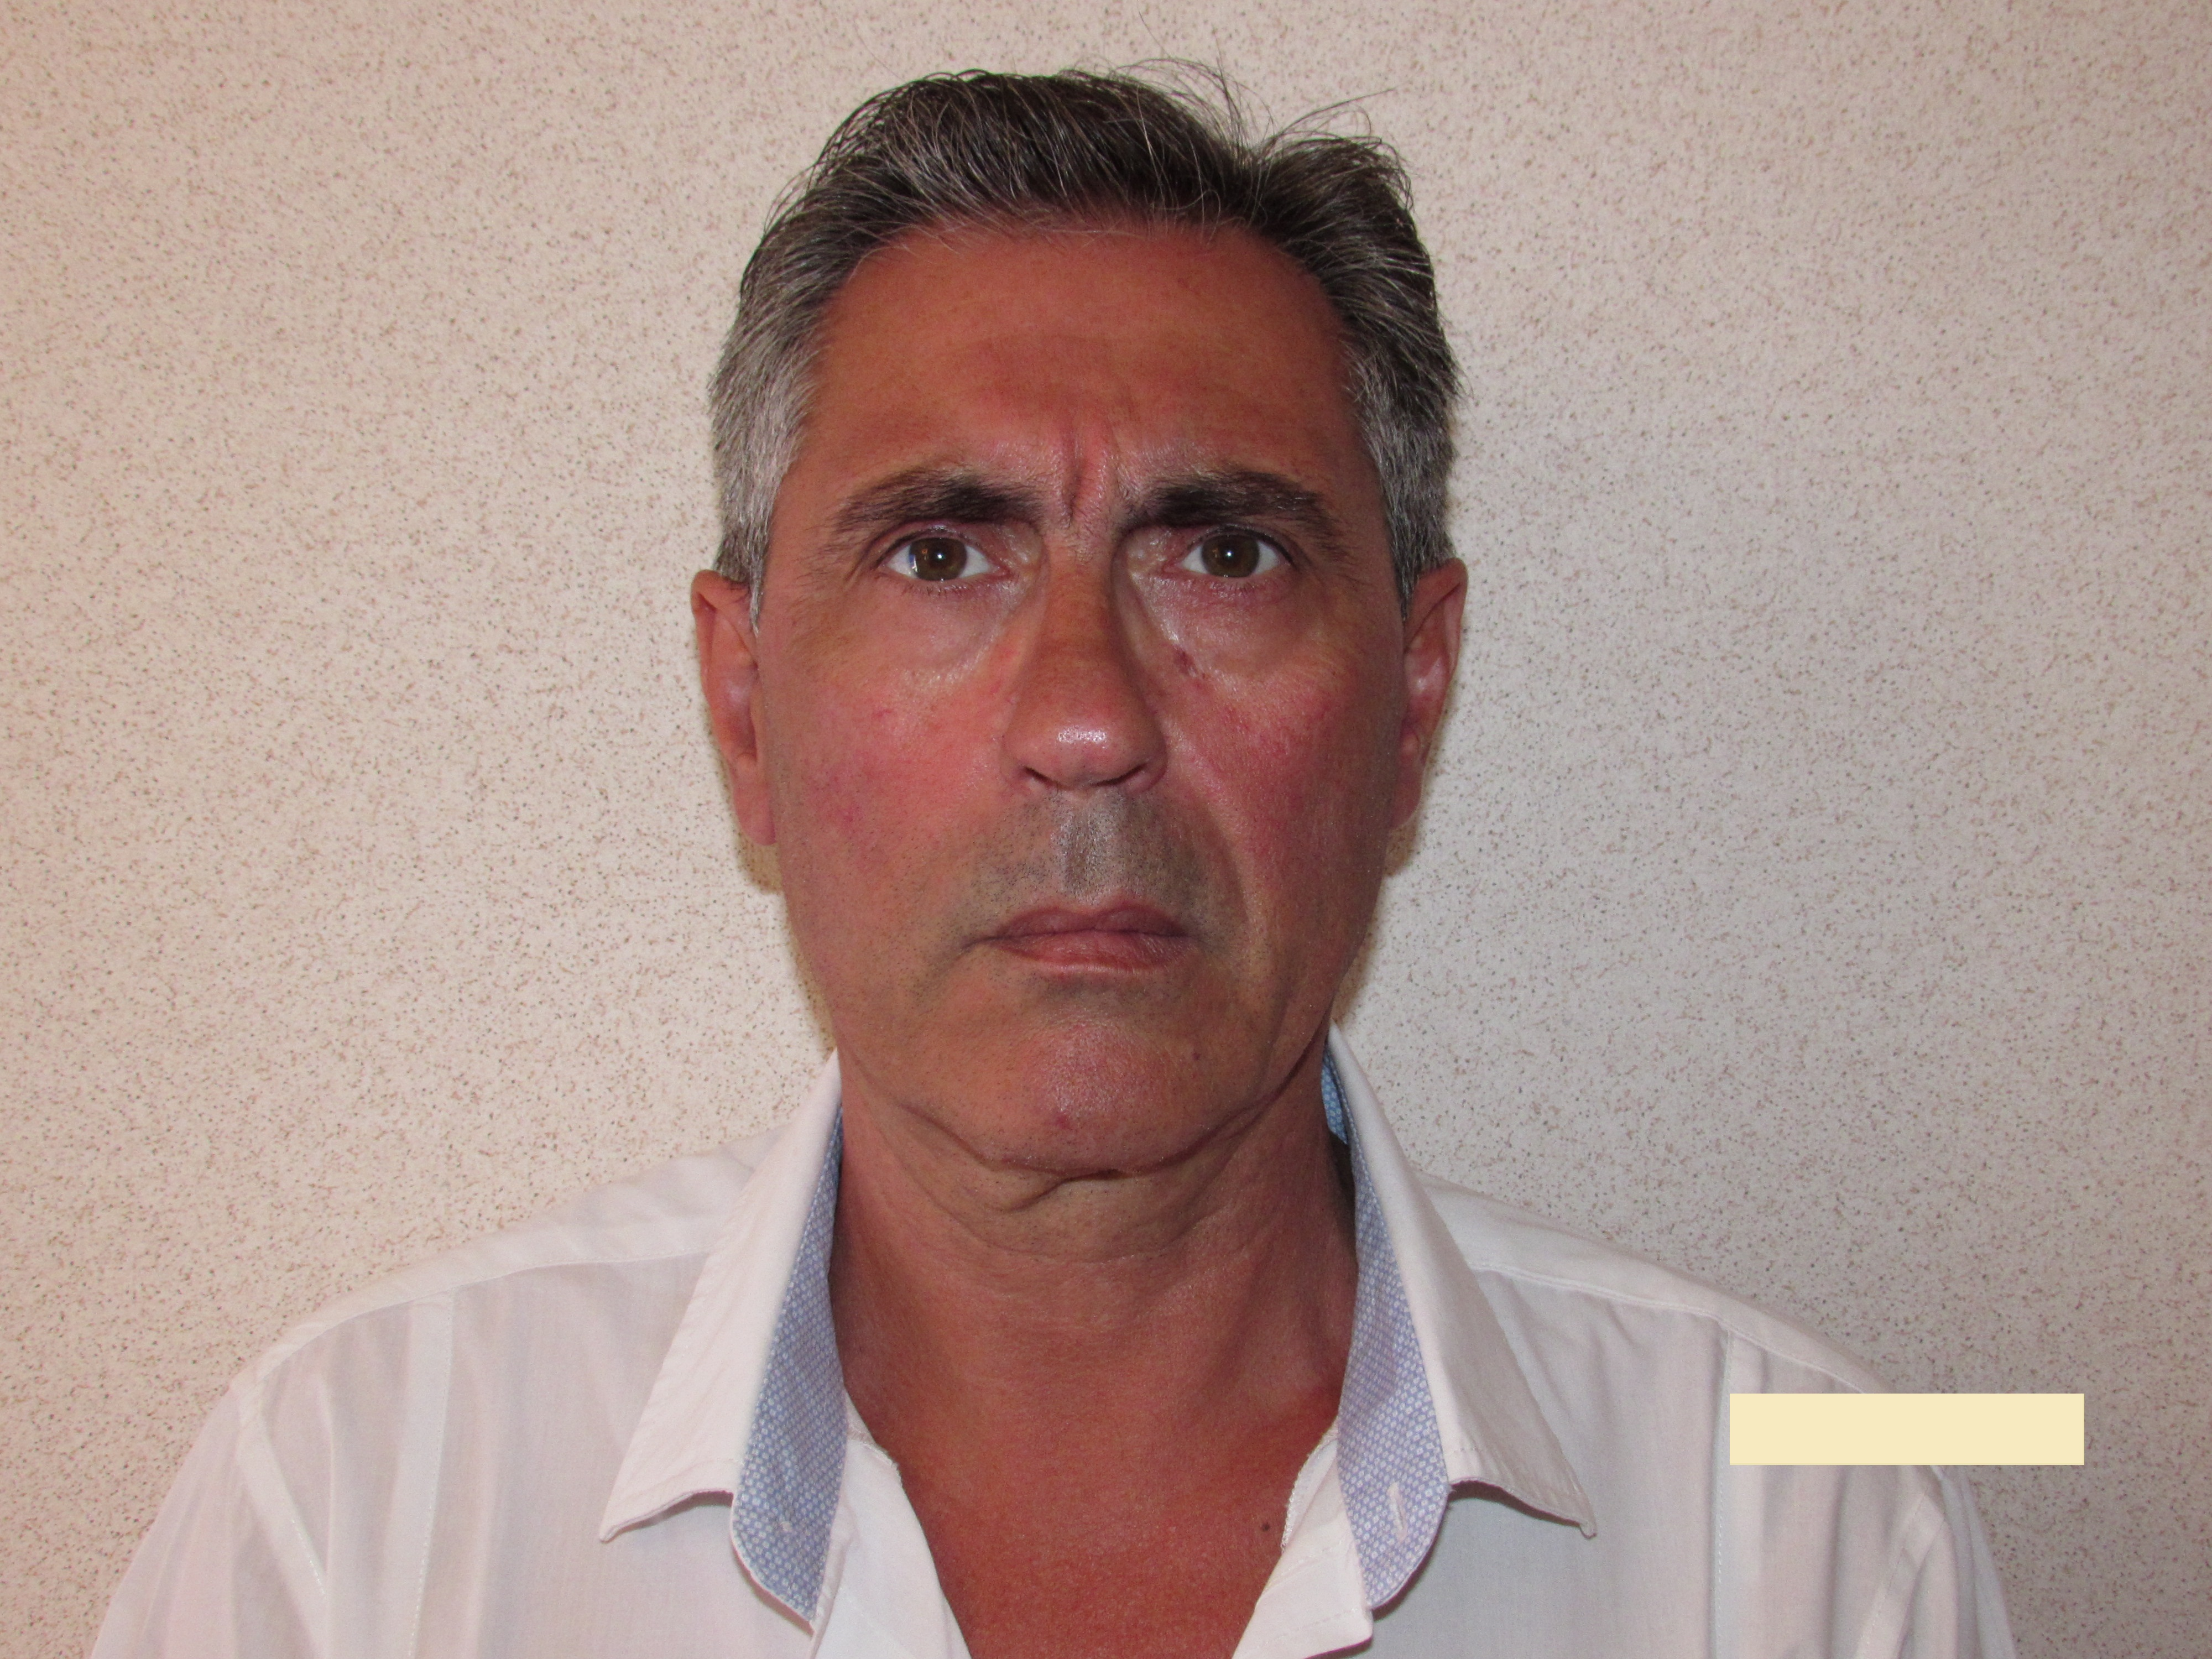
\includegraphics[height=.3\textheight]{figures/GIL-img6.jpg}

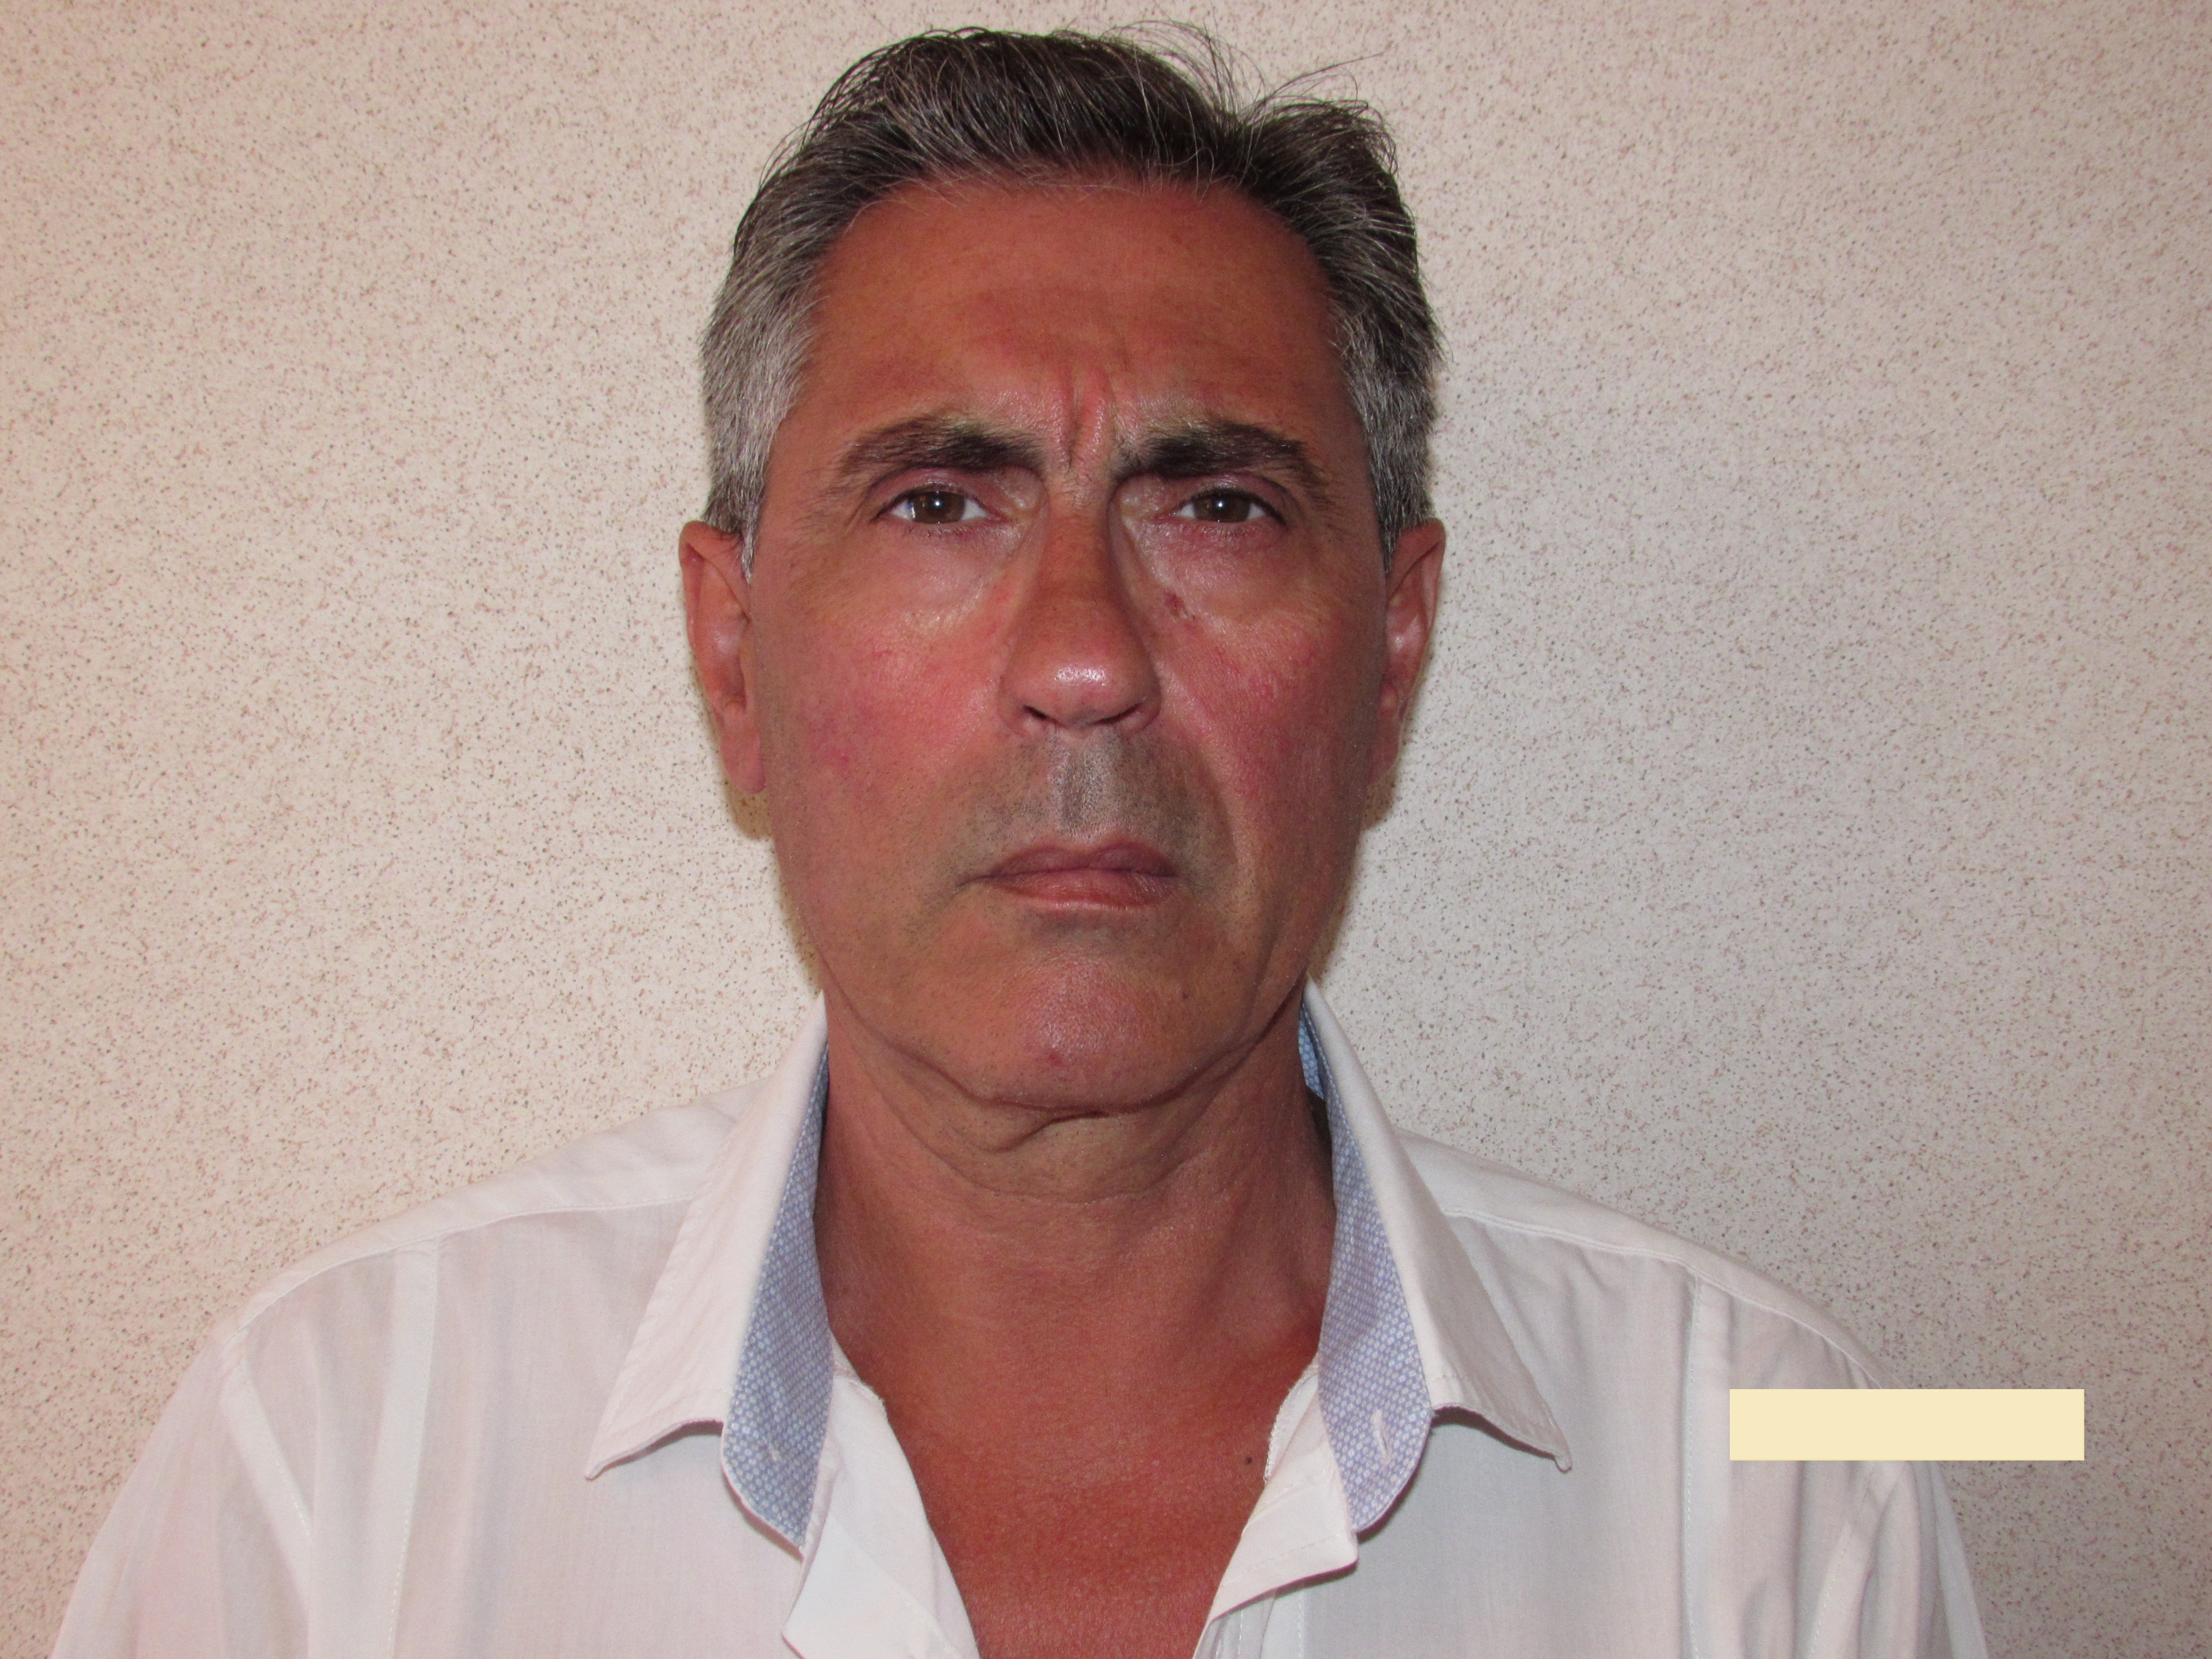
\includegraphics[height=.3\textheight]{figures/GIL-img7.jpg}

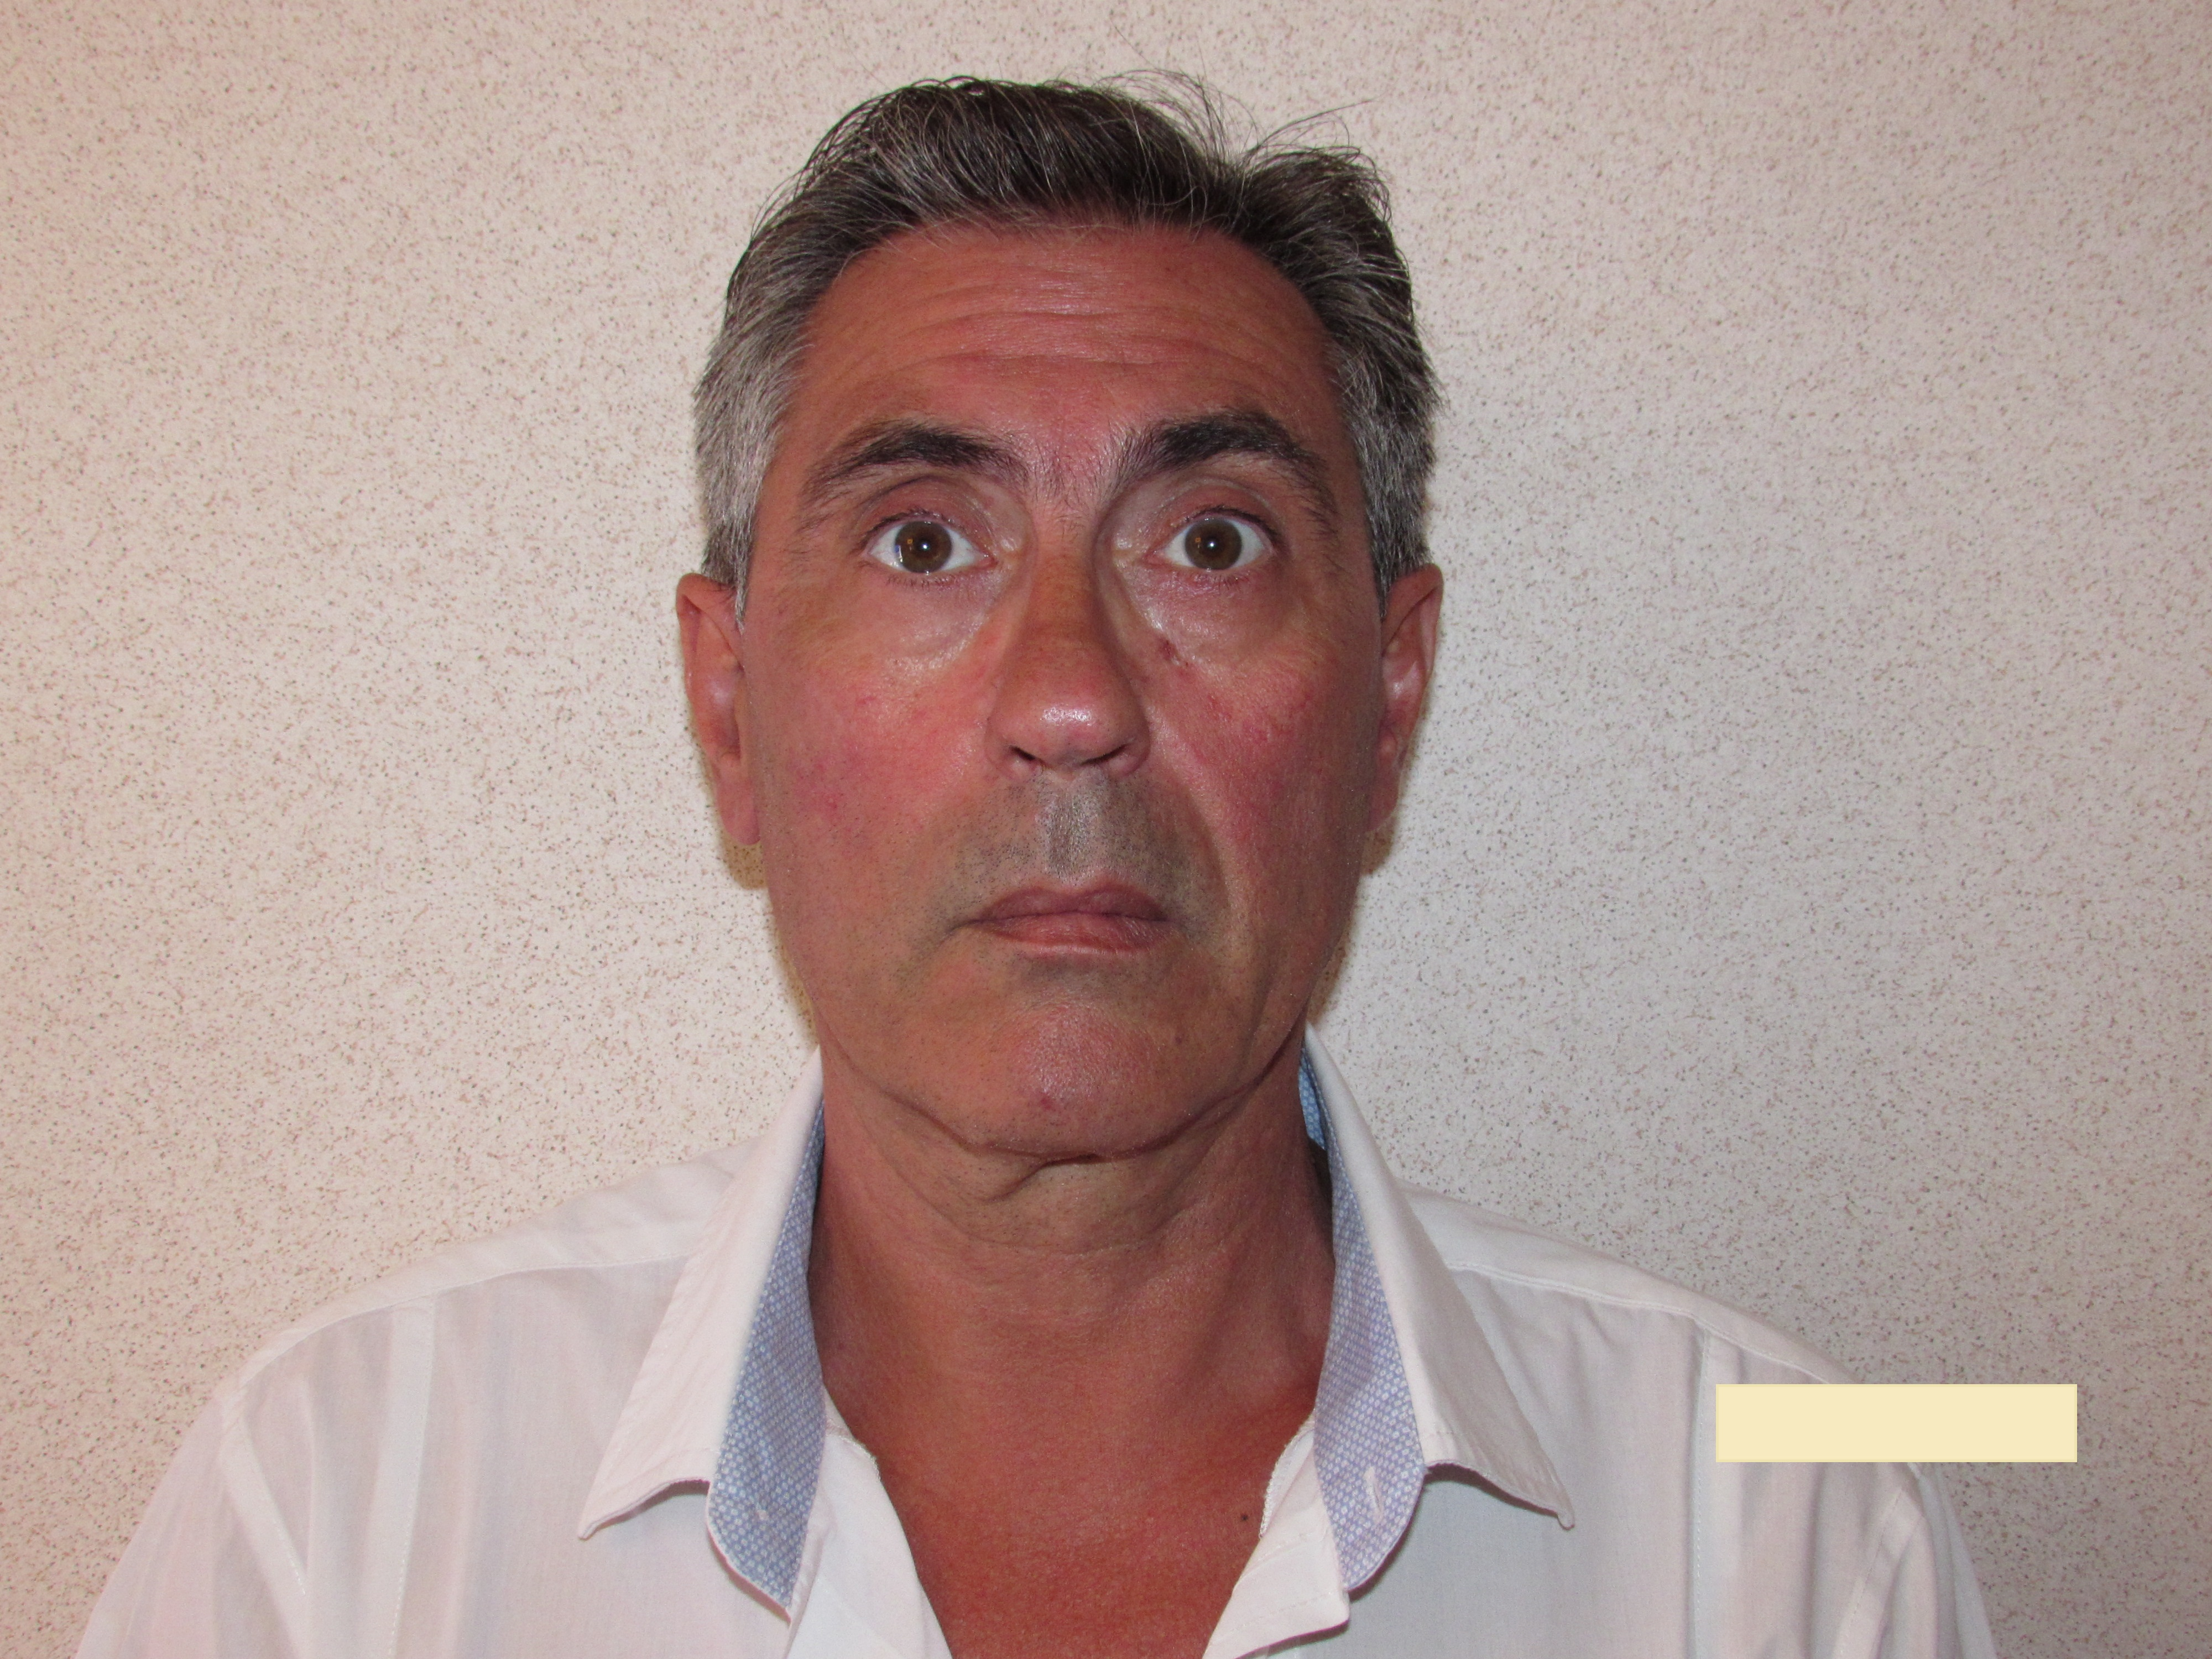
\includegraphics[height=.3\textheight]{figures/GIL-img8.jpg}
\caption{Examples of coding of Action Units involving Brows: AU4 \textup{Brow Lowerer} (first picture) or AU4+7 \textup{Brow Lowerer} + \textup{Lid Tightener} (second picture) and AU2 - \textup{Outer Brow Raiser (third picture)}.}
\label{fig:gil:4}
\end{figure} 

The coding system has been used even quite recently to label \isi{visual information} related to \isi{prosodic information} that clearly plays a linguistic role. For instance, in both the previously mentioned works by \citet{CrespoSendra2013} and \citet{GiliFivela2015informazionimultimodali}, after the recording of audio-video material (to be then used in perception experiments) a coding of the main patterns of facial expressions observed during the target utterances (usually on the nuclear accented word) was given. For instance, \citet[6]{CrespoSendra2013} report that\largerpage

\begin{quote}
for information-seeking interpretations the most common facial expression consisted of a combination of action units AU1 + 2 (Inner and Outer Brow Raisers) and head movement M59 (Head Down and Head Up). For incredulity question interpretations, the most common pattern was a combination of AU4 (Brow Lowered), M59 + 58 (Head Down and Head Back) and squinting of the eyes.
(\citealt[6]{CrespoSendra2013})
\end{quote}

On the contrary, in her work on statements, wh-questions conveying surprise and exclamations, \citet{GiliFivela2015informazionimultimodali} analyzes all the recorded audio-video sequences and labels the following main patterns in terms of FACS : 

\begin{itemize}
\item  for statements, AU0 - \textit{Neutral face} and AU M69 – \textit{Head and\slash or Eyes Look at Other} or M59 - \textit{Head Shake Up and Down} 
\item  for wh-questions (surprise and positive attitude), AU4+7 - \textit{Brow Lowerer} + \textit{Lid Tightener} or AU2 - \textit{Outer Brow Raiser}  and M60 - \textit{Head Shake Side to Side} 
\item  in exclamations (positive attitude), AU2 - \textit{Outer Brow Raiser} or AU4 - \textit{Brow Lowerer} and M59 - \textit{Head Shake Up and Down}. 
\end{itemize}

Results show a clear difference in \isi{eyebrow} and lid gestures when comparing neutral statements and other sentence modalities, while wh-questions expressing surprise and exclamations (both underlying positive attitude) show \isi{eyebrow} and lid gestures which are not always easily distinguishable (e.g., eyebrows rising or lowering usually take place in both questions and exclamations produced with a positive attitude, possibly with \textit{Lid tightening} in questions). On the other hand, results show that head movements seem to be similar in statements and exclamations \textit{(with head shaking up or down),} while wh-questions differ more clearly (because usually accompanied by \textit{head shaking side to side}). 

Therefore, the analysis of \isi{visual information} is performed with reference to a well-known coding system, with the aim of finding a correlation between \isi{prosodic} sound features and \isi{visual prosody} in expressing \isi{linguistic information}. However, take note that the FACS coding system would require more than one coder\slash \isi{transcriber} to analyze the data and, moreover, more than one coder\slash \isi{transcriber} which was officially trained in using the FACS coding system (for which \isi{inter-transcriber agreement} thresholds are known too). To the author's knowledge, this methodological procedure, in particular as for the official training, has not been really followed in works on linguistic \isi{prosody}, probably due to practical reasons. However, as for the number of transcribers, the situation brings to mind what is required for the coding of \isi{intonation} patterns within the ToBI system or with the coding of Map-Task dialogues, for which having more than one \isi{transcriber} would be methodologically correct and for which, not surprisingly, \isi{inter-transcriber agreement} thresholds have also been proposed in the literature (\citealt{Silverman1992,Beckman1997,Isard.Carletta1995}).\clearpage

\subsection{Advantages and disadvantages of the methods presented}\label{sec:gil:2:3}\largerpage
As for the use of optotracking systems, magnetometers or electromagnetic articulographs, the advantages, of course, relate to the chance of observing the articulatory correlates of \isi{prosody} (e.g., lengthening or strengthening phenomena) together with the timing of other articulatory and acoustic events (e.g. the timing of F0 peaks). This allows investigators to propose and refine models of gestural dynamics related to linguistically relevant \isi{prosodic} events and, the other way around, to consider linguistically relevant \isi{prosodic} events as related to gestural dynamics too.

For instance, thanks to the articulatory investigation \citet{Byrd1998} showed that various levels of \isi{prosodic} boundaries are distinguished by the temporal and spatial characteristics of articulatory gestures adjacent to the boundaries. In such a model, which is further developed in a following paper (\citealt{Byrd2003}), they propose that this lengthening is related to a specific \isi{prosodic} \isi{gesture} that regulates the duration of gestures at \isi{prosodic} boundaries. Mentioning another work described above, it is the sum of acoustic and articulatory data that allows \citet{Avesani2007} to illustrate that \isi{syllable} and \isi{vowel} \isi{prominence} are somehow directly proportional to the length, the velocity and the displacement of lip closing gestures. Furthermore, these data allow the authors to relate their results to a mass-spring gestural model (\citealt{Browman1995,Fowler1995,Saltzman1995,Saltzman1989}), arguing that, at least for one out of the two speakers considered, results can be accounted for by a single mechanism of linear rescaling. Thanks to both articulatory and acoustic data, \citet{Stella2014} show that in the three languages they considered the investigated acoustic tonal targets have a quite stable alignment with articulatory gestures. Moreover, they argue that results may be related to the \textit{Coupled Oscillator Model} of \isi{speech production} \citep{Goldstein2009}, and that the rising tonal \isi{gesture} would be in anti-phase relation with both the consonantal and the vocalic \isi{gesture}.

Disadvantages relate to the heaviness of data collection, which has an impact on both the number of speakers who are usually recorded and the complexity of data analysis; these aspects, of course, affect the whole experimental design, as they orient the choice of \isi{speech style} and corpus to be recorded. These first observations especially apply to data collection by means of articulographs, though the number of speakers considered in the studies has been gradually increasing over years. Moreover, the time required on average for the set-up, needed for gluing the sensors onto the subjects, both outside and inside the mouth, and the quite frequent event of a detachment of the glued sensor during data collection, make the whole recording phase time-consuming and challenging for both subjects and experimenter. In this respect, recording by means of diverse systems has various consequences as big differences may regard different versions of the same system (e.g., AG500 is far more instable than the new AG501 -- \citealt{Stella2012,Stella2013} -- and therefore it is obviously more difficult to record bigger corpora by means of the former than the latter). Whatever the system is, it is obviously true that recording articulatory data is more challenging than acquiring acoustic data only (sometimes even because of the difficulties in recruiting subjects willing to have electrodes glued, say, in their mouth).\largerpage

Moreover, data collected in articulatory studies usually correspond to very controlled speech material. Though, especially now that more stable machines are available, dialogical speech involving two speakers is collected by means of two systems at the same time (e.g., \citealt{Geng2013}), in most cases, data acquisition consists in exploiting one system and collecting very controlled, read speech data (e.g., see experiments described in the previous section). In fact, a single coil\slash articulator trajectory is extremely sensitive to the segmental environment not only in the sense that it may be modified by co-articulation, as expected and as observed for segments in acoustic data. The relevant point here is that it is the single coil\slash articulator to be investigated (e.g. lower lip, tongue dorsum) and in order to be able to observe its trajectories it is necessary to ensure the presence of significant (detectable) gestures from and to not adjacent segments. In this respect, segmental contexts that would not be problematic in acoustic investigations (where reaching of the set of expected articulatory targets in the sequence may ensure the necessary acoustic information) are in fact very problematic in articulatory investigations. For instance, given a pseudoword such as [mimi], thus including bilabial consonants produced by means of lip and jaw gestures, the tongue dorsum position for [i] will only slightly vary, and the risk is to be unable to unambiguously detect a significant tongue \isi{gesture} in the [i]-to-[i] cycle; thus, an [a]-to-[i] cycle would be preferable such as in [mami] or [mima]. Of course, these constraints do not have an impact only on investigations of segments. As exemplified in the experiments described in the previous sections, they are relevant in \isi{prosodic} investigations too, where reference to segments is usually needed and target words are usually chosen in order to satisfy the above-mentioned basic requirements.

Finally, labelling, measurements and data analysis relate to various sensors (e.g., tongue dorsum for \isi{vowel} articulation and lower lip for bilabial consonant) and axes (e.g. the z-axis for vertical movement and the x-axis for front-back horizontal movement). This means that a specific software is needed for labelling and measurements (e.g., HADES mentioned in relation to Byrd \& Saltzman’s \citeyear{Byrd1998} paper, \textit{Interface} mentioned in relation to \citealt{Avesani2007,Avesani2009} works, or MAYDAY, which was developed at CRIL for dealing with both kinematic data and ultrasound images, \citealt{Sigona2015}); moreover, it means that the amount of data is not easy to manage, especially when it also has to be related to data on acoustic \isi{prosody}, e.g. to F0 changes.

Turning to the imaging techniques, they also imply advantages and disadvantages. Gaining a wider view of the interaction between audio and \isi{visual information} may shed light on relevant factors that affect linguistic meaning and that are usually not taken into account in linguistic investigations. For instance, \citet{GiliFivela2015informazionimultimodali} reports a clear difference in \isi{eyebrow} and lid gestures when comparing neutral statements and the other sentence modalities considered, while underlining a similarity in the head movements observed during statements and exclamations. These observations may actually be of help when considering the phonological coding of intonational events. For instance, wh-questions are quite often found to be phonologically identical to statements (e.g., various contributions in \citealt{frotaPrieto2015}, starting from the paper on \ili{Italian}, i.e. \citealt{GiliFivelaETAL2015intonationalvariation}). Multimodal investigations may show that the adoption of the same \isi{intonational pattern} in statements and wh-questions could be problematic because of a number of other cues that speakers may use to distinguish statements from questions, among which visual cues could be considered besides, say, lexical and syntactic ones. That is, in the long run, a wider perspective in investigating speech may offer hints on the impact of \isi{visual information} on the variation observed in speech in general, as for both pattern choice and \isi{phonetic} implementation.

As for the disadvantages,  the use of cameras for acquiring both audio and video may imply a loss in the acoustic signal quality. The choice is then taken to be more appropriate when no accurate and extensive acoustic measurements or manipulations are performed. Another possible disadvantage may relate to criteria for subject selection, as some of the subjects, especially those who may already have troubles in immerging themselves in the given context during audio-recordings, may be even more clumsy if they know that video-recording is going on.\largerpage

\section{Perception} \label{sec:gil:3}
\subsection{Introduction} \label{sec:gil:3:1}
Investigations regarding the integration of \isi{audio-visual information} in the perception of \isi{prosody} have been strongly influenced by works on the McGurk effect, that is, on the integration of visual and auditory information which are not always consistent. 

In their \citeyear{McGurk1976} work, McGurk \& MacDonald asked their subjects to judge stimuli corresponding to the production of syllables [ba], [da], [ga], playing through a \isi{talking head} both stimuli in which either audio or video was available and stimuli in which both audio and video were available, though they were not always congruent (that is, for instance, both the audio and the \isi{visual information} corresponded to the production of [ba] or the audio corresponded to [ba] while the video showed the \isi{lip movement} for [ga]). Of course, attention was paid to the realization of stimuli that seemed as natural as possible, and indeed, as the authors stated, 

\begin{quote}
Dubbing was carried out so as to ensure, within the temporal constraints of telerecording equipment, that there was auditory-visual coincidence of the release of the consonant in the first \isi{syllable} of each utterance (\citealt[746]{McGurk1976}.)
\end{quote}

In particular, results of perception of stimuli in which the audio corresponded to [ba] while the \isi{lip movement} was that corresponding to [ga], showed that listeners reported hearing [da]; moreover, when subjects were presented the audio for [ga] on to the \isi{lip movement} for [ba], apart from [da], they mainly reported hearing [gabga], [bagba], [baga] or [gaba]. The authors argued that in the [ba]-audio\slash [ga]-video condition the acoustics for [ba] had features shared with [da] but not with [ga], that the \isi{visual information} was consistent with both [ga] and [da] and that, therefore, subjects were sensitive to the common information in both modalities. 

The influence of \isi{visual information} on the perception of \isi{audio information} reported by McGurk \& MacDonald represented a milestone in the investigation of multimodal perception, with clear methodological and theoretical impacts. Such impacts are considered in the following sections as for their influence on the investigation of \isi{prosody} in more recent studies, that basically started from the end of the 90s (see \citealt{Lansing1999} on the identification of statements vs. questions on the basis of visual cues in the upper facial regions and the observation that the recognition of \isi{prosodic information} from visual cues alone was more difficult than that of auditory cues).

Before addressing the specific methods adopted in the case of multimodal analyses, it is worth recalling that the focus here is the perception of \isi{linguistic information} conveyed by \isi{prosody}: methods to unimodally investigate this issue are quite well-known and are also used for multimodal investigations. For instance, identification and discrimination tests are used in checking for the existence of \isi{categorical perception} which, on the basis of the perception of segments, and consonants in particular (\citealt{Liberman1957}; see the contradicting results for vowels by \citealt{FryDB1962}), has been often taken to be a property of phonological (linguistic) units. In particular, specific characteristics are often expected in the identification of linguistically relevant sounds in that, in a traditional \isi{categorical perception paradigm} such as the one proposed for consonants by Liberman and colleagues in 1957, given a continuum of stimuli, when subjects are asked to identify the linguistic category they belong to, results are expected to be S-shaped, with a sharp switch from the perception of a category to the perception of another one; when subjects are asked to discriminate the same stimuli, that is they are given pairs or triplets of those stimuli and asked to judge whether some of them are equal or not, they are expected to be more sensitive to differences across categories, that is difference between intermediate stimuli in an S-shaped plot.\footnote{Of course these expectations are in line with a quantal theory of speech (\citealt{Stevens1972,Stevens1989}; see also \citealt{Stevens2010}), according to which categories correspond to quantal regions, clearly different from each other and whose members show acoustic and auditory characteristics which are quite stable, despite changes in articulatory settings. However, it is worth recalling that, following works on natural categories and their corresponding semantic categories (\citealt[193]{Rosch1975}; see also e.g. \citealt{Berlin1969}) showing that members of a category do not necessarily share an equal degree of membership, some works on segmental phonological categories \citep{Kuhl1991} and on \isi{intonation} categories too (\citealt{SchneiderEtAl2006,Schneider2009,GiliFivela2012}) addressed issues concerning the presence of prototypes or best examples, assuming the existence of non-homogenous categories - including prototypes - and the possibility to perceive differences in meaning or shades of meaning within a category \citep{GiliFivela2012}.} The existence of \isi{categorical perception} has been investigated with respect to \isi{intonation} categories too, adopting the same methods and formulating the same hypothesis, but reaching quite contradicting results which are more in line with those obtained for the perception of vowels (e.g., see the contradictory results reported by \citealt{Vanrell2006,SchneiderEtAl2006} and \citealt{Niebuhr2004}, and the discussion in the latter). A discussion of methods to unimodally investigate \isi{prosody} and \isi{intonation}, and for instance to design identification and discrimination tests is out of the scope of the present paper (but see, for instance, \citealt{Gussenhoven1999discreteness.gradience,Gussenhoven2004,GiliFivela2008book,Prieto.2012}) However, it is worth remembering that at least identification tests are often used in investigating multimodal perception too (see the next section) and that a possible distinction drawn among the various methods used to investigate the perception of \isi{prosody} may be useful to understand the criteria of selection of methods considered here. In particular, as proposed by \citet{GiliFivela2008book}, it is possible to distinguish methods for collecting subject’s metalinguistic judgements and procedures for directly recording speaker’s response and action taking. Among the former, methods are included requiring judgements on perceptual equivalence of stimuli, on successful imitation, asking for \isi{prominence} judgements, for semantic differences, semantic scaling, goodness rating, matching, as well as in identification and discrimination in \isi{categorical perception} paradigms; among the latter, methods are included asking for imitating stimuli, collecting eye tracking data, asking to perform games using audio stimuli and, in general, methods including reaction time measurements (for discussion, \citealt{GiliFivela2008book}). 

For space limits, in what follows only some methods relying on subjects’ metalinguistic judgements are basically referred to (e.g., investigations on neurophysiological correlates of multimodal perception are not discussed). 
 
\subsection{Methods for data collection and analysis: some examples} \label{sec:gil:3:2}
Data collection usually involves base stimuli including both audio and video, though this information may either be natural (audio and video taken from recording of speaker’s production) or synthetic (audio corresponding to synthetic \linebreak speech and video relating to computer-animated heads, that is \is{talking head}talking heads). Synthetic stimuli are necessarily used when continua are investigated and need to be judged by speakers. In these cases, both audio and video continua (typically representing the shift between two categories) may be created and synchronized with each other or one continuum may be created, e.g., the audio one, and synchronized with a sort of neutral condition on the other channel, e.g., regarding \isi{visual information}. In other cases, audio-video natural recordings are used, and the manipulation usually aims at crossing audio and visual conditions, rather than at realizing continua of changes. In these cases, the audio and video signals in the original recordings are separated via software, offering audio files and video clips that can be used as stimuli in audio-only and video-only tasks and that can also be crossed to obtain incongruent audio-visual stimuli, usually by creating all the possible combinations of audio and video cues. 

A check on the relevance of audio and \isi{visual information} is often carried out in investigations, with audio-only and video-only stimuli included in perception tests. However, in line with the traditional testing of the McGurk effect, the experimental procedure often also includes an explicit check for the \isi{audio-visual integration}, by means of audio-visual stimuli obtained by matching congruent and non-congruent audio and video information. 

In all cases, audio-visual stimuli are created by paying specific attention to the \isi{audio-visual information} synchronization, to create stimuli that are as natural as possible and that are free of artefacts.  Short pre-tests may indeed be used to check for the quality of stimuli. Stimuli are presented to subjects in random order, and usually in different blocks, and subjects are typically asked to perform an identification test and to judge whether stimuli are instances of one or another category. Reaction times in answering are measured in some investigations, and subjects may also be asked to score by means of Likert scales how confident they were when answering or how much they liked the specific item with respect to the category it was judged to belong to. Answers to (not manipulated) original recordings can be taken as control for every single subject or a control task may be included in the design, to check for subject comprehension of the task and stimuli.

For instance, \citet{House2002} investigates intonational cues and visual facial cues to the interrogative and statement mode in \ili{Swedish}. In a first experiment, he manipulates the acoustic information only, creating two sets of six stimuli in which the focal \isi{accent} peak is shifted and two F0 ranges for the focal \isi{accent} are considered. As for the \isi{visual information}, no head, eye or \isi{eyebrow} movement is visible in the \isi{talking head} presented to 11 subjects. On the basis of audio-visual stimuli, created by paying specific attention to the audio-visual synchronization, subjects are asked to judge whether the speaker intended to produce a statement or ask a question, and to mark on a 1-to-5 scale how much confident they are in their choice. However, in a second experiment, involving 27 subjects, the author uses the same audio stimuli, pairing them, in two different sets, with the movement configurations conveying either an interrogative (slow up-down head nod and \isi{eyebrow} lowering) or a \isi{declarative} mode (a smile throughout the whole utterance, a short up and down head nod and eye narrowing). The author can then demonstrate that the addition of the facial cues reinforces the information given by \isi{declarative} \isi{intonation} and inhibits that by the interrogative \isi{intonation}: basically, the interrogative face introduces more confusion to the perception of the stimuli and, subjects are less confident than when judging audio with no changing \isi{visual information}.

\citet{Srinivasan2003} analyze the perception of echoic questions and statements in English, presenting subjects with an auditory continuum that was crossed with a visual continuum, using \isi{synthetic speech} and a \isi{talking head}. In a first experiment, the authors present subjects with statement\slash question pairs in order to identify the pair which was best discriminated and used the acoustic and visual parameters of that pair as prototypical in order to synthesize the stimuli to be used for investigating \isi{audio-visual integration}. They used \textit{Wavesurfer} (\citealt{Sjolander.1999}) for investigating the acoustic parameters and a speech software tool called \textit{MarkupGUI} \citep{Wouters1999} to modify the acoustic (\isi{pitch contour}, amplitude, duration) and visual (\isi{eyebrow}, head tilt) parameters. In the second experiment, sixteen subjects evaluate stimuli (4 sentence pairs, auditorily, visually and bimodaly), judging each of the conditions 16 times in two sessions (8 times per session). Finally, in a third experiment, the visual and \isi{prosodic} cues previously exploited are considered as useful to create synthetic versions of an ideal statement and an ideal question and are then varied independently of one another. This way a five step series is created so that it

\begin{quote}
becomes more question-like with changing \isi{pitch contour} (of the entire sentence), and increasing amplitude and duration (of the \isi{final syllable}). The visual continuum becomes more question-like with increasing \isi{eyebrow} raise and head tilt (\citealt[9]{Srinivasan2003}).
\end{quote}

Forty-three subjects judged the stimuli (8 repetitions) realized by means of the ‘Baldi’ synthetic \isi{talking head} and the Festival \isi{synthetic speech}. The authors report strong individual differences in the perception of auditory or visual cues and in general a stronger relevance of auditory cues (results were replicated in a follow-up experiment in which either the visual cues were doubled in magnitude or the auditory cues were more ambiguous, narrowing the range of variation in the statement-question continuum)

Turning to \ili{Romance} languages, more recently, \citet{BorrasComes2011} describe two perception experiments in which stimuli, represented by manipulated speech and\slash or video signal, are used to test the integration of audio and \isi{visual information} and, in particular, the interaction of intonational and gestural information in the distinction between counter-expectational questions and \is{focus!narrow}narrow focus statements; a second goal is to identify the facial gestures conveying the \isi{counter-expectation interpretation}. To reach the first goal, the authors use an acoustic continuum representing the shift, in \ili{Catalan}, from a typical \is{focus!narrow}narrow focus statement to a typical  counter-expectational question (which are both realized with a \isi{rising pitch accent} followed by a \isi{low boundary tone}); as for \isi{visual information}, a continuum of facial gestures is created by means of a 3D animated character, tuning its movements in order to represent different levels of activation of an incredulity expression. In a second experiment, subjects judge stimuli composed by video information only, corresponding to animated sequences in which the same 3D character conveys incredulity in 4 different levels of activation by means of the three main gestures involved, that is \isi{brow} furrowing, eyelid closure and backward head movement, in all possible combinations. In both experiments stimuli are presented in random order by means of the software E-prime to eighteen \ili{Catalan} listeners, who judge 5 blocks of stimuli. The subjects have to express their preference as for the interpretation of the utterances and the software also collects their response times apart from the response frequencies. As for the interaction of audio and \isi{visual information}, results described by \citet{BorrasComes2011} show that the impact of \isi{intonation} decreases as the visual \isi{counter-expectation interpretation} information is clearer. The relevance of both audio and \isi{visual information} is shown by reaction time measurements, as \isi{intonation} has a great impact on them but it also interacts with gestures. However, as the second experiment shows, brow furrowing is crucial in distinguishing counter-expectation questions from \isi{narrow focus} statements when dependent on facial \isi{gesture} information, but subjects also rely on the other visual features (that appear to be given a specific degree of importance: brow furrowing > backward head movement > eyelid closure). 

In terms of methods adopted to collected perception data, audio-video recordings are also used in the literature, rather than \is{talking head}talking heads, together with a manipulation solely aimed at crossing audio and visual conditions rather than at realizing continua of changes.

To propose some examples,  \citet{CrespoSendra2013}, as already mentioned, record audio-visual material in order to create stimuli for a \isi{perception experiment}. The final aim is to compare the interaction between \isi{intonation} and facial gestures in the expression of information-seeking and incredulity yes\slash no questions in \ili{Catalan} and Dutch. The authors check for the \isi{audio-visual integration} by means of audio-video stimuli, and for the contribution of both audio and video by means of audio-only and video-only stimuli. The audio and video signals in the original recordings are separated (by means of the software Adobe Premiere), the audio files and the video clips are then used as stimuli in the audio-only and video-only tasks respectively. As for the audio-video task, original recordings are used as congruent stimuli, while non-congruent stimuli are obtained by manipulating the audio-video signals (with the above-mentioned software). Manipulation consists in matching, for each speaker, all the possible combinations of audio and video cues for the various interpretations (e.g., neutral face-incredulous \isi{intonation} and incredulous face-neutral \isi{intonation}). Once  a pre-test of the material ensures their \isi{naturalness} and lack of artefacts, the tests can take place (each preceded by a training phase).  \citet{CrespoSendra2013} ask their subjects to perform the video-only and audio-only test in a different order, and both before the audio-visual task, which is also preceded by a short documentary projection to avoid possible learning effects. In addition, they have a short final control task to confirm that the 10 audio-only and video-only stimuli (by a new speaker) are unambiguously interpreted by participants. All tasks are run by means of E-Prime. Thus, given a stimulus, subjects have to choose between a neutral and an incredulous information seeking question. The authors find that, in both languages, visual cues have a stronger impact than auditory cues to induce correct identification of incredulity in questions. However, languages differ as for the weight given to the cues. Indeed, as audio-video stimuli show, \ili{Catalan} listeners give more weight to facial cues than Dutch listeners. 

As a final example, \citet{GiliFivela2015informazionimultimodali}, as mentioned in \sectref{sec:gil:2:2}, investigates facial expressions across sentence modalities, considering wh-questions, statements and exclamations in \ili{Italian}. Similarly to  \citet{CrespoSendra2013}, the author checks for the \isi{audio-visual integration} by means of audio-only, video-only and audio-visual stimuli, including both congruent and incongruent stimuli. The procedure followed is very similar, apart from the fact that the separation of audio and video channel is performed by means of a public domain software, Virtual-Dub, a simple break is taken before the audio-visual task and the answers to (not manipulated) original recordings are taken as control for every single subject (no final control task is included in the design). The entire experiment is run by means of the software Presentation and subjects are asked both to choose between three options, which is a statement, a question and an \isi{exclamation}, and to rate on a 7-point Likert scale the negative-positive attitude of the speaker. The analysis of subject answers in favour of the three given options shows a fairly articulated picture and the lack of a systematic positive influence of video over audio or vice versa. In particular, video information related to neutral statements does not interfere with \isi{audio information}; on the contrary, video information regarding questions, and, though to a lesser extent, that related to exclamations affect the interpretation of the \isi{audio information} on neutral statements. 
 
\subsection{Advantages and disadvantages of the methods presented} \label{sec:gil:3:3}
The main advantage of the methods used to investigate the perception of \isi{multimodal information} is considered here to be, of course, the chance of observing both the audio and the visual correlates of \isi{prosody}, and the possibility of understanding how they are integrated. Moreover, some methodological choices allow to do so even in the case of artificial continua of variation. All in all, these methods allow to investigate the communication of \isi{prosody} as the multimodal phenomenon it usually is. However, results reported in the literature so far are quite composite and much work still needs to be done to really understand the issue. 

For instance, it was the investigation of \isi{audio-visual integration} that allowed \citet{House2002} to show that the addition of facial cues reinforced the information offered by \isi{declarative} \isi{intonation} only, while it inhibited the information related to interrogative \isi{intonation} (as the interrogative face introduced confusion to the perception of the stimuli). Along quite similar lines, by investigating both audio and \isi{visual information} \citet{BorrasComes2011} could show that the impact of \isi{intonation} decreased as the visual (\isi{counter-expectation interpretation}) information was clearer, while \citet{Srinivasan2003} could report a stronger relevance of auditory cues, apart from strong individual differences in the perception of auditory or visual cues.

Additionally, similar investigations can specifically emphasize the relationship between the quantity and quality of information in audio (in terms of \isi{phonetic} and phonological information available) and in video and their role in \isi{audio-visual integration}. For instance,  \citet{CrespoSendra2013} found that, in both \ili{Catalan} and Dutch, visual cues have a stronger impact than auditory cues to induce correct identification of incredulity in questions, though \ili{Catalan} listeners give more importance to visual cues than Dutch listeners, probably because of the more subtle distinction due to acoustic information in \ili{Catalan} (\isi{pitch range} difference) with respect to the information available in Dutch (where a different sequence of tonal events, that is a different set of phonological categories, characterize the contours of the utterances under investigation). Nevertheless, as \citet{GiliFivela2015informazionimultimodali} argues, the picture on the \isi{audio-visual integration} of information is quite articulated, and this may explain the lack of consistent results on a systematic positive influence of video over audio or vice versa. In particular, results on \ili{Italian} show that \isi{visual information} on surprised questions and exclamations affect the interpretation of \isi{audio information} on neutral statements, but not the other way around, independently of the information available on the audio channel (i.e. on the phonological pattern which was implemented). Thus, marked facial expressions and head movements (in her work associated to questions and exclamations) seem to affect the interpretation of utterances which are not associated to marked information on the same channel (in her work, neutral statements), rather than to affect information which is ambiguous in the other channel, that is sound.\largerpage[-1] 

Not surprisingly, then, these investigations possibly support different theories of speech perception, such as the single channel model (SCM), the weighted averaging model (WTAV) and the fuzzy logical model of perception (FLMP) (for a discussion, see \citealt{Massaro1989,MassaroCohen1993,Srinivasan2003}).\footnote{Briefly, according to the SCM only one of the auditory and visual channels of information is functional on any given bimodal input, that is, SCM is a non-integration model according to which a single channel of information can be processed at any one time. However, according to the other two models, different sources of information may be processed. According to the WTAV, they “are averaged according to the weight assigned to each modality” (\citealt[10]{Srinivasan2003}), while according to the FLMP the influence of one modality is going to be greater when the other is weaker and more ambiguous.} A discussion of the models is out of the scope of the present paper. However, it is worth mentioning here that \citet[20]{Srinivasan2003} found that the FLMP was not significantly better than the WTAV\slash SCM models, while \citet{BorrasComes2011} do not assume a clear position as for the model (WTAV or FLMP) that is better supported by their data, though they suggest that their results could be consistent with FLMP (especially for the relevance of both audio and \isi{visual information} shown by reaction time results). Along similar lines,  \citet{CrespoSendra2013} argue that their results agree with the FLMP, as an ambiguous or weaker cue in one modality seems to enhance the role of the other modality. However, \citet{GiliFivela2015informazionimultimodali} observes that her results seem to support the idea that it is not only the relation of information available in the channels that plays a role (e.g. the \isi{visual information} and the phonological pattern implemented and conveyed by means of the audio channel), but also the balancing of information within the same channel. Indeed,  the \isi{visual information} in questions (and partly in exclamations) affects the audio interpretation of statements, but not the other way around (visual in statements does not equally affect audio in questions). Thus, investigating the perception of multimodal \isi{prosodic information} is still needed to really answer the question concerning the role of audio and \isi{visual information} and the way they are integrated. Luckily, this can be done also by resorting to quite a high number of subjects for each \isi{perception experiment}, which makes results more solid and generalizable.

As for disadvantages related to the methods described here, it is important to underline that they correspond to difficulties rather than to real disadvantages. As a matter of fact, one main difficulty is detected in data collection, mainly because of the need to ensure \isi{naturalness} in the stimuli used for perception experiments. This aspect brings us back to difficulties in collecting the speech material to be used to create stimuli, that is in eliciting as spontaneous and as natural sounding speech as possible (see \sectref{sec:gil:2:3}). However, the \isi{naturalness} of stimuli to be used in perception experiments also strongly depends on the manipulation procedures applied to cross the audio and \isi{visual information}. In this respect, the details given by \citet[746]{McGurk1976}\footnote{See citation reported above.}, already put the issue in the correct light, emphasizing the importance of the temporal alignment of auditory and \isi{visual information}. Even if the concern is not directly the segmental information, as in the original McGurk \& MacDonald investigation, this is an important matter any time a manipulation is necessary to match information conveyed by different channels, for instance, any time incongruous stimuli are created. In fact, the \isi{naturalness} of stimuli represents one of the most important factors to warrant the reliability of collected perceptual data. It may be important to keep the issue in mind even before the creation of incongruous stimuli, that is when the originals are segmented. Indeed, as  \citet[211]{GiliFivela2015informazionimultimodali} observes, generating files of very similar duration (and, in particular, audio-video composed by the same number of frames) and in which the utterance starts after a given time-interval from the starting point of the file may be of great help in facilitating the best match when modifying the pairing of the two channels in order to generate the various audio-video combinations. Of course, the utterance duration itself within the file may be another issue as, even warranting the same starting point in the production of speech and \isi{visual information}, a problem may relate to the matching of the utterance length and this may require some extra manipulation. Moreover, particularly when considering \isi{visual information} and \isi{prosody} or, more specifically, \isi{intonation}, explicit attention has to be devoted to the alignment of visual and \isi{audio information} when pitch accents are realized, as the peaking of \isi{visual information} aligned with pitch accents is reported in the literature (e.g., \citealt{Cassell1994,Loehr2004,Swerts2008}). So the manipulation phase is very delicate and a final check on the \isi{naturalness} of stimuli is needed to warrant the results of perception data collection.

\section{Conclusions}\label{sec:gil:4}
The paper offers an overview of the methods used in the literature on \isi{prosody} and \isi{intonation} to perform multimodal analyses of audio-visual material conveying \isi{linguistic information} in speech. Importantly, as for \isi{visual information}, the paper discusses both articulatory gestures directly involved in the production of speech (e.g., lip gestures) and information that may be more traditionally considered and referred to as speech accompanying gestures (focusing on head movements and visual expressions). 

Methods adopted to investigate \isi{speech production} and perception are considered, by mainly describing experimental designs of works focusing mainly on \ili{Italian} and some other \ili{Romance} languages. The quite detailed description of methods offered in sections \ref{sec:gil:2:2} and \ref{sec:gil:3:2} aims at emphasizing the key aspects allowing the reader to choose among the various methods and aims at offering the relevant references for their deeper understanding.  Additionally, it represents a necessary, preliminary step to discuss advantages and disadvantages related to the different methodological choices, both by highlighting very practical issues or drawbacks related to them and by stressing their impact in terms of theoretical issues and models they are used to refer to.

In very general terms, \isi{visual information} as a whole may be taken to belong to the extralinguistic context the speakers resort to in order to understand messages and optimize them in production. However, some specific \isi{visual information} clearly participates in conveying strictly \isi{linguistic information}, such as \isi{sentence modality} (see \sectref{sec:gil:2:2}). The relevance of such visual cues with respect to the audio ones is still to be understood (e.g., see \sectref{sec:gil:3:3}). However, the importance of resorting to both audio and visual cues is quite clear when thinking of most communication going on in everyday life. Moreover, it is clear also in specific situations. For instance, it is possible to create different local contexts in which the ``truth value" of an utterance changes, by exploiting the flow of information in the channels or modalities available to the speakers (that is audio-only or audio-video, as discussed by \citealt{GiliFivela2014} and recalled at the beginning of the paper -- see \sectref{sec:gil:1}). 

The examples discussed and the possible specific suggestions given in the paper are in line with the idea that multimodal analyses of multimodal, \isi{audio-visual information} may be useful in order not only to understand the relation between the various sources of information we usually exploit in communication {per se}, but also to shed a possible new light on the variability otherwise observed in acoustic and articulatory investigation of speech material. The \isi{visual information} may indeed represent an extra factor to be considered, besides those usually focused on in linguistic investigations, such as the lexical and syntactic make-up of utterances. Indeed, it may shed light on the variation observed in speech as for both pattern choice and \isi{phonetic} implementation. Along this line of reasoning, it is plausible that the relevance of \isi{visual information} could also play a role in relation to the differences observed in the perception of members of the same categories. In this respect, the existence of prototypes and non-prototypes, also mentioned in relation to the perception of \isi{intonation} categories (e.g., \citealt{Schneider2005,SchneiderEtAl2006,Schneider2009,GiliFivela2012}; see \fnref{fn:gil:2} in \sectref{sec:gil:3:1}), could also turn out to be relevant to the issue. Indeed, a non-prototypical member of a category, judged because of its acoustic characteristics, may actually be judged differently once that \isi{visual information} is also considered. This would be in line with the possibility to resort to intra-category variability to express shades of meanings by means of the modulation of acoustic and, possibly, \isi{visual information} too.

{
\sloppy
\printbibliography[heading=subbibliography,notkeyword=this]
}
\end{document}
